\section{A Tour Through RCU's Requirements}
\label{sec:rcu:A Tour Through RCU's Requirements}

\begin{Note}
Copyright IBM Corporation, 2015

Author: Paul E. McKenney

The initial version of this document appeared in the
\href{https://lwn.net/}{LWN} on those articles:
\href{https://lwn.net/Articles/652156/}{part 1},
\href{https://lwn.net/Articles/652677/}{part 2}, and
\href{https://lwn.net/Articles/653326/}{part 3}.
\end{Note}


\subsection{Introduction}

Read-copy update (RCU) is a synchronization mechanism that is often used
as a replacement for reader-writer locking.
RCU is unusual in that
updaters do not block readers, which means that RCU's read-side
primitives can be exceedingly fast and scalable.
In addition, updaters
can make useful forward progress concurrently with readers.
However, all
this concurrency between RCU readers and updaters does raise the
question of exactly what RCU readers are doing, which in turn raises the
question of exactly what RCU's requirements are.

This document therefore summarizes RCU's requirements, and can be
thought of as an informal, high-level specification for RCU\@.
It is
important to understand that RCU's specification is primarily empirical
in nature; in fact, I learned about many of these requirements the hard
way.
This situation might cause some consternation, however, not only
has this learning process been a lot of fun, but it has also been a
great privilege to work with so many people willing to apply
technologies in interesting new ways.

All that aside, here are the categories of currently known RCU
requirements:

\begin{enumerate}
\item Fundamental Requirements
\item Fundamental Non-Requirements
\item Parallelism Facts of Life
\item Quality-of-Implementation Requirements
\item Linux Kernel Complications
\item Software-Engineering Requirements
\item Other RCU Flavors
\item Possible Future Changes
\end{enumerate}

This is followed by a summary.

%however, the answers to
%each quick quiz immediately follows the quiz.
%Select the big white space
%with your mouse to see the answer.

\begin{Note}
  Quick Quizzes are rendered by perfbook's scheme, where the answers
  go to a later chapter.
  Each pair of quiz and answer is cross-referenced by hyper-links in
  the PDF\@.
\end{Note}

\subsection{Fundamental Requirements}

RCU's fundamental requirements are the closest thing RCU has to hard
mathematical requirements.
These are:

\begin{enumerate}
\item Grace-Period Guarantee
\item Publish/Subscribe Guarantee
\item Memory-Barrier Guarantees
\item RCU Primitives Guaranteed to Execute Unconditionally
\item Guaranteed Read-to-Write Upgrade
\end{enumerate}

\subsubsection{Grace-Period Guarantee}

RCU's grace-period guarantee is unusual in being premeditated:
Jack
Slingwine and I had this guarantee firmly in mind when we started work
on RCU (then called “rclock”) in the early 1990s.
That said, the past
two decades of experience with RCU have produced a much more detailed
understanding of this guarantee.

RCU's grace-period guarantee allows updaters to wait for the completion
of all pre-existing RCU read-side critical sections.
An RCU read-side
critical section begins with the marker \co{rcu_read_lock()} and ends
with the marker \co{rcu_read_unlock()}.
These markers may be nested, and
RCU treats a nested set as one big RCU read-side critical section.
Production-quality implementations of \co{rcu_read_lock()} and
\co{rcu_read_unlock()} are extremely lightweight, and in fact have
exactly zero overhead in Linux kernels built for production use with
\co{CONFIG_PREEMPTION=n}.

This guarantee allows ordering to be enforced with extremely low
overhead to readers, for example:

\begin{VerbatimN}
	int x, y;

	void thread0(void)
	{
		rcu_read_lock();
		r1 = READ_ONCE(x);
		r2 = READ_ONCE(y);
		rcu_read_unlock();
	}

	void thread1(void)
	{
		WRITE_ONCE(x, 1);
		synchronize_rcu();
		WRITE_ONCE(y, 1);
	}
\end{VerbatimN}

Because the \co{synchronize_rcu()} on \clnref{} % line 14
waits for all pre-existing
readers, any instance of \co{thread0()} that loads a value of zero
from~\co{x} must complete before \co{thread1()} stores to~\co{y}, so that
instance must also load a value of zero from~\co{y}.
Similarly, any
instance of \co{thread0()} that loads a value of one from~\co{y} must have
started after the \co{synchronize_rcu()} started, and must therefore also
load a value of one from~\co{x}.
Therefore, the outcome:

\begin{VerbatimU}
	(r1 == 0 && r2 == 1)
\end{VerbatimU}

\noindent%
cannot happen.

\QuickQuiz{
  Wait a minute!
  You said that updaters can make useful forward
  progress concurrently with readers, but pre-existing readers will
  block \co{synchronize_rcu()}!!!
  Just who are you trying to fool???
}\QuickQuizAnswer{
  First, if updaters do not wish to be blocked by readers, they can use
  \co{call_rcu()} or \co{kfree_rcu()}, which will be discussed later.
  Second, even when using \co{synchronize_rcu()}, the other update-side
  code does run concurrently with readers, whether pre-existing or not.
}\QuickQuizEnd

This scenario resembles one of the first uses of RCU in
\href{https://en.wikipedia.org/wiki/DYNIX}{DYNIX/ptx}, which managed a
distributed lock manager's transition into a state suitable for handling
recovery from node failure, more or less as follows:

\begin{VerbatimN}
       1 #define STATE_NORMAL        0
       2 #define STATE_WANT_RECOVERY 1
       3 #define STATE_RECOVERING    2
       4 #define STATE_WANT_NORMAL   3
       5
       6 int state = STATE_NORMAL;
       7
       8 void do_something_dlm(void)
       9 {
      10   int state_snap;
      11
      12   rcu_read_lock();
      13   state_snap = READ_ONCE(state);
      14   if (state_snap == STATE_NORMAL)
      15     do_something();
      16   else
      17     do_something_carefully();
      18   rcu_read_unlock();
      19 }
      20
      21 void start_recovery(void)
      22 {
      23   WRITE_ONCE(state, STATE_WANT_RECOVERY);
      24   synchronize_rcu();
      25   WRITE_ONCE(state, STATE_RECOVERING);
      26   recovery();
      27   WRITE_ONCE(state, STATE_WANT_NORMAL);
      28   synchronize_rcu();
      29   WRITE_ONCE(state, STATE_NORMAL);
      30 }
\end{VerbatimN}

The RCU read-side critical section in \co{do_something_dlm()} works with
the \co{synchronize_rcu()} in \co{start_recovery()} to guarantee that
\co{do_something()} never runs concurrently with \co{recovery()}, but with
little or no synchronization overhead in \co{do_something_dlm()}.

\QuickQuiz{
  Why is the \co{synchronize_rcu()} on \clnref{} %line 28
  needed?
}\QuickQuizAnswer{
  Without that extra grace period, memory reordering could result in
  \co{do_something_dlm()} executing \co{do_something()} concurrently with
  the last bits of \co{recovery(}.
}\QuickQuizEnd

In order to avoid fatal problems such as deadlocks, an RCU read-side
critical section must not contain calls to \co{synchronize_rcu()}.
Similarly, an RCU read-side critical section must not contain anything
that waits, directly or indirectly, on completion of an invocation of
\co{synchronize_rcu()}.

Although RCU's grace-period guarantee is useful in and of itself, with
\href{https://lwn.net/Articles/573497/}{quite a few use cases}, it would
be good to be able to use RCU to coordinate read-side access to linked
data structures.
For this, the grace-period guarantee is not sufficient,
as can be seen in function \co{add_gp_buggy()} below.
We will look at the
reader's code later, but in the meantime, just think of the reader as
locklessly picking up the \co{gp} pointer, and, if the value loaded is
non-\co{NULL}, locklessly accessing the \co{->a} and \co{->b} fields.

\begin{VerbatimN}
       1 bool add_gp_buggy(int a, int b)
       2 {
       3   p = kmalloc(sizeof(*p), GFP_KERNEL);
       4   if (!p)
       5     return -ENOMEM;
       6   spin_lock(&gp_lock);
       7   if (rcu_access_pointer(gp)) {
       8     spin_unlock(&gp_lock);
       9     return false;
      10   }
      11   p->a = a;
      12   p->b = a;
      13   gp = p; /* ORDERING BUG */
      14   spin_unlock(&gp_lock);
      15   return true;
      16 }
\end{VerbatimN}

The problem is that both the compiler and weakly ordered CPUs are within
their rights to reorder this code as follows:

\begin{VerbatimN}
       1 bool add_gp_buggy_optimized(int a, int b)
       2 {
       3   p = kmalloc(sizeof(*p), GFP_KERNEL);
       4   if (!p)
       5     return -ENOMEM;
       6   spin_lock(&gp_lock);
       7   if (rcu_access_pointer(gp)) {
       8     spin_unlock(&gp_lock);
       9     return false;
      10   }
      11   gp = p; /* ORDERING BUG */
      12   p->a = a;
      13   p->b = a;
      14   spin_unlock(&gp_lock);
      15   return true;
      16 }
\end{VerbatimN}

If an RCU reader fetches \co{gp} just after \co{add_gp_buggy_optimized}
executes \clnref{}, % line 11
it will see garbage in the \co{->a} and \co{->b} fields.
And this is but one of many ways in which compiler and hardware
optimizations could cause trouble.
Therefore, we clearly need some way
to prevent the compiler and the CPU from reordering in this manner,
which brings us to the publish-subscribe guarantee discussed in the next
section.

\subsubsection{Publish/Subscribe Guarantee}

RCU's publish-subscribe guarantee allows data to be inserted into a
linked data structure without disrupting RCU readers.
The updater uses
\co{rcu_assign_pointer()} to insert the new data, and readers use
\co{rcu_dereference()} to access data, whether new or old.
The following
shows an example of insertion:

\begin{VerbatimN}
       1 bool add_gp(int a, int b)
       2 {
       3   p = kmalloc(sizeof(*p), GFP_KERNEL);
       4   if (!p)
       5     return -ENOMEM;
       6   spin_lock(&gp_lock);
       7   if (rcu_access_pointer(gp)) {
       8     spin_unlock(&gp_lock);
       9     return false;
      10   }
      11   p->a = a;
      12   p->b = a;
      13   rcu_assign_pointer(gp, p);
      14   spin_unlock(&gp_lock);
      15   return true;
      16 }
\end{VerbatimN}

The \co{rcu_assign_pointer()} on \clnref{} % line 13
is conceptually equivalent to a
simple assignment statement, but also guarantees that its assignment
will happen after the two assignments in \clnref{,}, %lines 11 and 12
similar to the
C11 \co{memory_order_release} store operation.
It also prevents any
number of ``interesting'' compiler optimizations, for example, the use of
\co{gp} as a scratch location immediately preceding the assignment.

\QuickQuiz{
  But \co{rcu_assign_pointer()} does nothing to prevent the two
  assignments to \co{p->a} and \co{p->b} from being reordered.
  Can't that
  also cause problems?
}\QuickQuizAnswer{
  No, it cannot. The readers cannot see either of these two fields
  until the assignment to \co{gp}, by which time both fields are fully
  initialized.
  So reordering the assignments to \co{p->a} and \co{p->b}
  cannot possibly cause any problems.
}\QuickQuizEnd

It is tempting to assume that the reader need not do anything special to
control its accesses to the RCU-protected data, as shown in
\co{do_something_gp_buggy()} below:

\begin{VerbatimN}
       1 bool do_something_gp_buggy(void)
       2 {
       3   rcu_read_lock();
       4   p = gp;  /* OPTIMIZATIONS GALORE!!! */
       5   if (p) {
       6     do_something(p->a, p->b);
       7     rcu_read_unlock();
       8     return true;
       9   }
      10   rcu_read_unlock();
      11   return false;
      12 }
\end{VerbatimN}

However, this temptation must be resisted because there are a
surprisingly large number of ways that the compiler (or weak ordering
CPUs like the DEC Alpha) can trip this code up.
For but one example, if
the compiler were short of registers, it might choose to refetch from
\co{gp} rather than keeping a separate copy in~\co{p} as follows:

\begin{VerbatimN}
       1 bool do_something_gp_buggy_optimized(void)
       2 {
       3   rcu_read_lock();
       4   if (gp) { /* OPTIMIZATIONS GALORE!!! */
       5     do_something(gp->a, gp->b);
       6     rcu_read_unlock();
       7     return true;
       8   }
       9   rcu_read_unlock();
      10   return false;
      11 }
\end{VerbatimN}

If this function ran concurrently with a series of updates that replaced
the current structure with a new one, the fetches of \co{gp->a}n and
\co{gp->b} might well come from two different structures, which could
cause serious confusion.
To prevent this (and much else besides),
\co{do_something_gp()} uses \co{rcu_dereference()} to fetch from \co{gp}:

\begin{VerbatimN}
       1 bool do_something_gp(void)
       2 {
       3   rcu_read_lock();
       4   p = rcu_dereference(gp);
       5   if (p) {
       6     do_something(p->a, p->b);
       7     rcu_read_unlock();
       8     return true;
       9   }
      10   rcu_read_unlock();
      11   return false;
      12 }
\end{VerbatimN}

The \co{rcu_dereference()} uses volatile casts and (for DEC Alpha) memory
barriers in the Linux kernel.
Should a
\href{http://www.rdrop.com/users/paulmck/RCU/consume.2015.07.13a.pdf}
{high-quality implementation of C11 \co{memory_order_consume} [PDF]}
ever appear, then \co{rcu_dereference()} could be implemented as a
\co{memory_order_consume} load. Regardless of the exact implementation, a
pointer fetched by \co{rcu_dereference()} may not be used outside of the
outermost RCU read-side critical section containing that
\co{rcu_dereference()}, unless protection of the corresponding data
element has been passed from RCU to some other synchronization
mechanism, most commonly locking or reference counting
(see \path{../../rcuref.rst}).

In short, updaters use \co{rcu_assign_pointer()} and readers use
\co{rcu_dereference()}, and these two RCU API elements work together to
ensure that readers have a consistent view of newly added data elements.

Of course, it is also necessary to remove elements from RCU-protected
data structures, for example, using the following process:

\begin{enumerate}
\item Remove the data element from the enclosing structure.
\item Wait for all pre-existing RCU read-side critical sections to complete
   (because only pre-existing readers can possibly have a reference to
   the newly removed data element).
\item At this point, only the updater has a reference to the newly removed
   data element, so it can safely reclaim the data element, for example,
   by passing it to \co{kfree()}.
\end{enumerate}

This process is implemented by \co{remove_gp_synchronous()}:

\begin{VerbatimN}
       1 bool remove_gp_synchronous(void)
       2 {
       3   struct foo *p;
       4
       5   spin_lock(&gp_lock);
       6   p = rcu_access_pointer(gp);
       7   if (!p) {
       8     spin_unlock(&gp_lock);
       9     return false;
      10   }
      11   rcu_assign_pointer(gp, NULL);
      12   spin_unlock(&gp_lock);
      13   synchronize_rcu();
      14   kfree(p);
      15   return true;
      16 }
\end{VerbatimN}

This function is straightforward, with \clnref{} % line13
waiting for a grace
period before \clnref % line 14
frees the old data element.
This waiting ensures
that readers will reach \clnref{} % line 7
of \co{do_something_gp()} before the data
element referenced by~\co{p} is freed.
The \co{rcu_access_pointer()} on \clnref{} % line 6
is similar to \co{rcu_dereference()}, except that:

\begin{enumerate}
\item The value returned by \co{rcu_access_pointer()} cannot be
   dereferenced. If you want to access the value pointed to as well as
   the pointer itself, use \co{rcu_dereference()} instead of
   \co{rcu_access_pointer()}.
\item The call to \co{rcu_access_pointer()} need not be protected.
   In
   contrast, \co{rcu_dereference()} must either be within an RCU
   read-side critical section or in a code segment where the pointer
   cannot change, for example, in code protected by the corresponding
   update-side lock.
\end{enumerate}

\QuickQuiz{
  Without the \co{rcu_dereference()} or the \co{rcu_access_pointer()},
  what destructive optimizations might the compiler make use of?
}\QuickQuizAnswer{
  Let's start with what happens to \co{do_something_gp()} if it fails to
  use \co{rcu_dereference()}.
  It could reuse a value formerly fetched
  from this same pointer.
  It could also fetch the pointer from \co{gp}
  in a byte-at-a-time manner, resulting in \emph{load tearing}, in turn
  resulting a bytewise mash-up of two distinct pointer values.
  It might
  even use value-speculation optimizations, where it makes a wrong
  guess, but by the time it gets around to checking the value, an
  update has changed the pointer to match the wrong guess.
  Too bad
  about any dereferences that returned pre-initialization garbage in
  the meantime!
  For \co{remove_gp_synchronous()}, as long as all modifications to
  \co{gp} are carried out while holding \co{gp_lock}, the above
  optimizations are harmless.
  However, \co{sparse} will complain if you
  define \co{gp} with \co{__rcu} and then access it without using either
  \co{rcu_access_pointer()} or \co{rcu_dereference()}.
}\QuickQuizEnd

In short, RCU's publish-subscribe guarantee is provided by the
combination of \co{rcu_assign_pointer()} and \co{rcu_dereference()}.
This
guarantee allows data elements to be safely added to RCU-protected
linked data structures without disrupting RCU readers.
This guarantee
can be used in combination with the grace-period guarantee to also allow
data elements to be removed from RCU-protected linked data structures,
again without disrupting RCU readers.

This guarantee was only partially premeditated.
DYNIX/ptx used an
explicit memory barrier for publication, but had nothing resembling
\co{rcu_dereference()} for subscription, nor did it have anything
resembling the dependency-ordering barrier that was later subsumed
into \co{rcu_dereference()} and later still into \co{READ_ONCE()}.
The
need for these operations made itself known quite suddenly at a
late-1990s meeting with the DEC Alpha architects, back in the days when
DEC was still a free-standing company.
It took the Alpha architects a
good hour to convince me that any sort of barrier would ever be needed,
and it then took me a good \emph{two} hours to convince them that their
documentation did not make this point clear.
More recent work with the C
and C++ standards committees have provided much education on tricks and
traps from the compiler.
In short, compilers were much less tricky in
the early 1990s, but in 2015, don't even think about omitting
\co{rcu_dereference()}!


\subsubsection{Memory-Barrier Guarantees}

The previous section's simple linked-data-structure scenario clearly
demonstrates the need for RCU's stringent memory-ordering guarantees on
systems with more than one CPU\@:

\begin{enumerate}
\item Each CPU that has an RCU read-side critical section that begins
   before \co{synchronize_rcu()} starts is guaranteed to execute a full
   memory barrier between the time that the RCU read-side critical
   section ends and the time that \co{synchronize_rcu()} returns.
   Without
   this guarantee, a pre-existing RCU read-side critical section might
   hold a reference to the newly removed \co{struct foo} after the
   \co{kfree()} on \clnref{} % line 14
   of \co{remove_gp_synchronous()}.
\item Each CPU that has an RCU read-side critical section that ends after
   \co{synchronize_rcu()} returns is guaranteed to execute a full memory
   barrier between the time that \co{synchronize_rcu()} begins and the
   time that the RCU read-side critical section begins.
   Without this
   guarantee, a later RCU read-side critical section running after the
   \co{kfree()} on \clnref{} % line 14
   of \co{remove_gp_synchronous()} might later run
   \co{do_something_gp()} and find the newly deleted \co{struct foo}.
\item If the task invoking \co{synchronize_rcu()} remains on a given CPU,
   then that CPU is guaranteed to execute a full memory barrier sometime
   during the execution of \co{synchronize_rcu()}.
   This guarantee ensures
   that the \co{kfree()} on \clnref{} % line 14
   of \co{remove_gp_synchronous()} really
   does execute after the removal on \clnref{}. % line 11
\item If the task invoking \co{synchronize_rcu()} migrates among a group of
   CPUs during that invocation, then each of the CPUs in that group is
   guaranteed to execute a full memory barrier sometime during the
   execution of \co{synchronize_rcu()}.
   This guarantee also ensures that
   the \co{kfree()} on \clnref{} % line 14
   of \co{remove_gp_synchronous()} really does
   execute after the removal on \clnref{}, % line 11
   but also in the case where the
   thread executing the \co{synchronize_rcu()} migrates in the meantime.
\end{enumerate}

\QuickQuiz{
  Given that multiple CPUs can start RCU read-side critical sections at
  any time without any ordering whatsoever, how can RCU possibly tell
  whether or not a given RCU read-side critical section starts before a
  given instance of \co{synchronize_rcu()}?
}\QuickQuizAnswer{
  If RCU cannot tell whether or not a given RCU read-side critical
  section starts before a given instance of \co{synchronize_rcu()}, then
  it must assume that the RCU read-side critical section started first.
  In other words, a given instance of \co{synchronize_rcu()} can avoid
  waiting on a given RCU read-side critical section only if it can
  prove that \co{synchronize_rcu()} started first.
  A related question is ``When \co{rcu_read_lock()} doesn't generate any
  code, why does it matter how it relates to a grace period?''
  The
  answer is that it is not the relationship of \co{rcu_read_lock()}
  itself that is important, but rather the relationship of the code
  within the enclosed RCU read-side critical section to the code
  preceding and following the grace period.
  If we take this viewpoint,
  then a given RCU read-side critical section begins before a given
  grace period when some access preceding the grace period observes the
  effect of some access within the critical section, in which case none
  of the accesses within the critical section may observe the effects
  of any access following the grace period.

  As of late 2016, mathematical models of RCU take this viewpoint, for
  example, see slides 62 and 63 of the
  \href{http://www2.rdrop.com/users/paulmck/scalability/paper/LinuxMM.2016.10.04c.LCE.pdf}{2016 LinuxCon}
  presentation.
}\QuickQuizEnd

\QuickQuiz{
  The first and second guarantees require unbelievably strict ordering!
  Are all these memory barriers \emph{really} required?
}\QuickQuizAnswer{
  Yes, they really are required.
  To see why the first guarantee is
  required, consider the following sequence of events:

  \begin{enumerate}
  \item CPU 1: \co{rcu_read_lock()}
  \item CPU 1: \co{q = rcu_dereference(gp); /* Very likely to return p. */}
  \item CPU 0: \co{list_del_rcu(p);}
  \item CPU 0: \co{synchronize_rcu()} starts.
  \item CPU 1: \co{do_something_with(q->a);} \\
     \co{/* No smp_mb(), so might happen after kfree(). */}
  \item CPU 1: \co{rcu_read_unlock()}
  \item CPU 0: \co{synchronize_rcu()} returns.
  \item CPU 0: \co{kfree(p);}
  \end{enumerate}

  Therefore, there absolutely must be a full memory barrier between the
  end of the RCU read-side critical section and the end of the grace
  period.

  The sequence of events demonstrating the necessity of the second rule
  is roughly similar:

  \begin{enumerate}
  \item CPU 0: \co{list_del_rcu(p);}
  \item CPU 0: \co{synchronize_rcu()} starts.
  \item CPU 1: \co{rcu_read_lock()}
  \item CPU 1: \co{q = rcu_dereference(gp);} \\
     \co{/* Might return p if no memory barrier. */}
  \item CPU 0: \co{synchronize_rcu()} returns.
  \item CPU 0: \co{kfree(p);}
  \item CPU 1: \co{do_something_with(q->a); /* Boom!!! */}
  \item CPU 1: \co{rcu_read_unlock()}
  \end{enumerate}

  And similarly, without a memory barrier between the beginning of the
  grace period and the beginning of the RCU read-side critical section,
  CPU~1 might end up accessing the freelist.

  The ``as if'' rule of course applies, so that any implementation that
  acts as if the appropriate memory barriers were in place is a correct
  implementation.
  That said, it is much easier to fool yourself into
  believing that you have adhered to the as-if rule than it is to
  actually adhere to it!
}\QuickQuizEnd

\QuickQuiz{
  You claim that \co{rcu_read_lock()} and \co{rcu_read_unlock()} generate
  absolutely no code in some kernel builds.
  This means that the
  compiler might arbitrarily rearrange consecutive RCU read-side
  critical sections.
  Given such rearrangement, if a given RCU read-side
  critical section is done, how can you be sure that all prior RCU
  read-side critical sections are done? Won't the compiler
  rearrangements make that impossible to determine?
}\QuickQuizAnswer{
  In cases where \co{rcu_read_lock()} and \co{rcu_read_unlock()} generate
  absolutely no code, RCU infers quiescent states only at special
  locations, for example, within the scheduler.
  Because calls to
  \co{schedule()} had better prevent calling-code accesses to shared
  variables from being rearranged across the call to \co{schedule()}, if
  RCU detects the end of a given RCU read-side critical section, it
  will necessarily detect the end of all prior RCU read-side critical
  sections, no matter how aggressively the compiler scrambles the code.
  Again, this all assumes that the compiler cannot scramble code across
  calls to the scheduler, out of interrupt handlers, into the idle
  loop, into user-mode code, and so on. But if your kernel build allows
  that sort of scrambling, you have broken far more than just RCU!
}\QuickQuizEnd

Note that these memory-barrier requirements do not replace the
fundamental RCU requirement that a grace period wait for all
pre-existing readers.
On the contrary, the memory barriers called out in
this section must operate in such a way as to \emph{enforce} this fundamental
requirement. Of course, different implementations enforce this
requirement in different ways, but enforce it they must.


\subsubsection{RCU Primitives Guaranteed to Execute Unconditionally}

The common-case RCU primitives are unconditional.
They are invoked, they
do their job, and they return, with no possibility of error, and no need
to retry.
This is a key RCU design philosophy.

However, this philosophy is pragmatic rather than pigheaded.
If someone
comes up with a good justification for a particular conditional RCU
primitive, it might well be implemented and added. After all, this
guarantee was reverse-engineered, not premeditated.
The unconditional
nature of the RCU primitives was initially an accident of
implementation, and later experience with synchronization primitives
with conditional primitives caused me to elevate this accident to a
guarantee.
Therefore, the justification for adding a conditional
primitive to RCU would need to be based on detailed and compelling use
cases.


\subsubsection{Guaranteed Read-to-Write Upgrade}

As far as RCU is concerned, it is always possible to carry out an update
within an RCU read-side critical section. For example, that RCU
read-side critical section might search for a given data element, and
then might acquire the update-side spinlock in order to update that
element, all while remaining in that RCU read-side critical section. Of
course, it is necessary to exit the RCU read-side critical section
before invoking \co{synchronize_rcu()}, however, this inconvenience can
be avoided through use of the \co{call_rcu()} and \co{kfree_rcu()} API
members described later in this document.

\QuickQuiz{
  But how does the upgrade-to-write operation exclude other readers?
}\QuickQuizAnswer{
  It doesn't, just like normal RCU updates, which also do not exclude
  RCU readers.
}\QuickQuizEnd

This guarantee allows lookup code to be shared between read-side and
update-side code, and was premeditated, appearing in the earliest
DYNIX/ptx RCU documentation.


\subsection{Fundamental Non-Requirements}

RCU provides extremely lightweight readers, and its read-side
guarantees, though quite useful, are correspondingly lightweight.
It is
therefore all too easy to assume that RCU is guaranteeing more than it
really is.
Of course, the list of things that RCU does not guarantee is
infinitely long, however, the following sections list a few
non-guarantees that have caused confusion.
Except where otherwise noted,
these non-guarantees were premeditated.

\begin{enumerate}
\item Readers Impose Minimal Ordering
\item Readers Do Not Exclude Updaters
\item Updaters Only Wait For Old Readers
\item Grace Periods Don't Partition Read-Side Critical Sections
\item Read-Side Critical Sections Don't Partition Grace Periods
\end{enumerate}


\subsubsection{Readers Impose Minimal Ordering}

Reader-side markers such as \co{rcu_read_lock()} and
\co{rcu_read_unlock()} provide absolutely no ordering guarantees except
through their interaction with the grace-period APIs such as
\co{synchronize_rcu()}.
To see this, consider the following pair of
threads:

\begin{VerbatimN}
       1 void thread0(void)
       2 {
       3   rcu_read_lock();
       4   WRITE_ONCE(x, 1);
       5   rcu_read_unlock();
       6   rcu_read_lock();
       7   WRITE_ONCE(y, 1);
       8   rcu_read_unlock();
       9 }
      10
      11 void thread1(void)
      12 {
      13   rcu_read_lock();
      14   r1 = READ_ONCE(y);
      15   rcu_read_unlock();
      16   rcu_read_lock();
      17   r2 = READ_ONCE(x);
      18   rcu_read_unlock();
      19 }
\end{VerbatimN}

After \co{thread0()} and \co{thread1()} execute concurrently, it is quite
possible to have

\begin{VerbatimU}
      (r1 == 1 && r2 == 0)
\end{VerbatimU}

\noindent%
(that is, \co{y}~appears to have been assigned before~\co{x}), which would
not be possible if \co{rcu_read_lock()} and \co{rcu_read_unlock()} had
much in the way of ordering properties.
But they do not, so the CPU is
within its rights to do significant reordering.
This is by design:
Any
significant ordering constraints would slow down these fast-path APIs.

\QuickQuiz{
  Can't the compiler also reorder this code?
}\QuickQuizAnswer{
  No, the volatile casts in \co{READ_ONCE()} and \co{WRITE_ONCE()}
  prevent the compiler from reordering in this particular case.
}\QuickQuizEnd


\subsubsection{Readers Do Not Exclude Updaters}

Neither \co{rcu_read_lock()} nor \co{rcu_read_unlock()} exclude updates.
All they do is to prevent grace periods from ending. The following
example illustrates this:

\begin{VerbatimN}
       1 void thread0(void)
       2 {
       3   rcu_read_lock();
       4   r1 = READ_ONCE(y);
       5   if (r1) {
       6     do_something_with_nonzero_x();
       7     r2 = READ_ONCE(x);
       8     WARN_ON(!r2); /* BUG!!! */
       9   }
      10   rcu_read_unlock();
      11 }
      12
      13 void thread1(void)
      14 {
      15   spin_lock(&my_lock);
      16   WRITE_ONCE(x, 1);
      17   WRITE_ONCE(y, 1);
      18   spin_unlock(&my_lock);
      19 }
\end{VerbatimN}

If the \co{thread0()} function's \co{rcu_read_lock()} excluded the
\co{thread1()} function's update, the \co{WARN_ON()} could never fire.
But
the fact is that \co{rcu_read_lock()} does not exclude much of anything
aside from subsequent grace periods, of which \co{thread1()} has none, so
the \co{WARN_ON()} can and does fire.


\subsubsection{Updaters Only Wait For Old Readers}

It might be tempting to assume that after \co{synchronize_rcu()}
completes, there are no readers executing.
This temptation must be
avoided because new readers can start immediately after
\co{synchronize_rcu()} starts, and \co{synchronize_rcu()} is under no
obligation to wait for these new readers.

\QuickQuiz{
  Suppose that \co{synchronize_rcu()} did wait until \emph{all} readers had
  completed instead of waiting only on pre-existing readers.
  For how
  long would the updater be able to rely on there being no readers?
}\QuickQuizAnswer{
  For no time at all.
  Even if \co{synchronize_rcu()} were to wait until
  all readers had completed, a new reader might start immediately after
  \co{synchronize_rcu()} completed.
  Therefore, the code following
  \co{synchronize_rcu()} can \emph{never} rely on there being no readers.
}\QuickQuizEnd


\subsubsection{Grace Periods Don't Partition Read-Side Critical Sections}

It is tempting to assume that if any part of one RCU read-side critical
section precedes a given grace period, and if any part of another RCU
read-side critical section follows that same grace period, then all of
the first RCU read-side critical section must precede all of the second.
However, this just isn't the case:
A single grace period does not
partition the set of RCU read-side critical sections.
An example of this
situation can be illustrated as follows, where \co{x}, \co{y}, and~\co{z}
are initially all zero:

\begin{VerbatimN}
       1 void thread0(void)
       2 {
       3   rcu_read_lock();
       4   WRITE_ONCE(a, 1);
       5   WRITE_ONCE(b, 1);
       6   rcu_read_unlock();
       7 }
       8
       9 void thread1(void)
      10 {
      11   r1 = READ_ONCE(a);
      12   synchronize_rcu();
      13   WRITE_ONCE(c, 1);
      14 }
      15
      16 void thread2(void)
      17 {
      18   rcu_read_lock();
      19   r2 = READ_ONCE(b);
      20   r3 = READ_ONCE(c);
      21   rcu_read_unlock();
      22 }
\end{VerbatimN}

It turns out that the outcome:

\begin{VerbatimU}
      (r1 == 1 && r2 == 0 && r3 == 1)
\end{VerbatimU}

\noindent%
is entirely possible.
The following figure show how this can happen,
with each circled \co{QS} indicating the point at which RCU recorded a
\emph{quiescent state} for each thread, that is, a state in which RCU knows
that the thread cannot be in the midst of an RCU read-side critical
section that started before the current grace period:

\begin{center}
\resizebox{.7\columnwidth}{!}{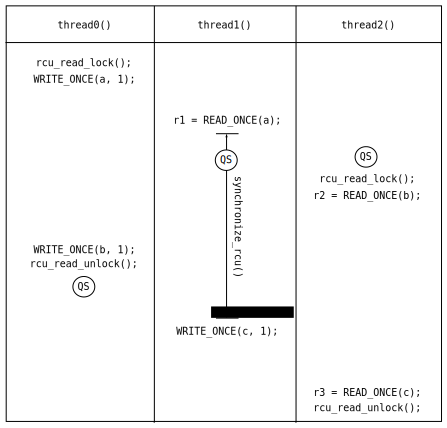
\includegraphics{rcu/design/GPpartitionReaders1}}
\end{center}

If it is necessary to partition RCU read-side critical sections in this
manner, it is necessary to use two grace periods, where the first grace
period is known to end before the second grace period starts:

\begin{VerbatimN}
       1 void thread0(void)
       2 {
       3   rcu_read_lock();
       4   WRITE_ONCE(a, 1);
       5   WRITE_ONCE(b, 1);
       6   rcu_read_unlock();
       7 }
       8
       9 void thread1(void)
      10 {
      11   r1 = READ_ONCE(a);
      12   synchronize_rcu();
      13   WRITE_ONCE(c, 1);
      14 }
      15
      16 void thread2(void)
      17 {
      18   r2 = READ_ONCE(c);
      19   synchronize_rcu();
      20   WRITE_ONCE(d, 1);
      21 }
      22
      23 void thread3(void)
      24 {
      25   rcu_read_lock();
      26   r3 = READ_ONCE(b);
      27   r4 = READ_ONCE(d);
      28   rcu_read_unlock();
      29 }
\end{VerbatimN}

Here, if \co{(r1 == 1)}, then \co{thread0()}'s write to~\co{b} must happen
before the end of \co{thread1()}'s grace period.
If in addition
\co{(r4 == 1)}, then \co{thread3()}'s read from~\co{b} must happen after
the beginning of \co{thread2()}'s grace period.
If it is also the case
that \co{(r2 == 1)}, then the end of \co{thread1()}'s grace period must
precede the beginning of \co{thread2()}'s grace period.
This mean that
the two RCU read-side critical sections cannot overlap, guaranteeing
that \co{(r3 == 1)}.
As a result, the outcome:

\begin{VerbatimU}
      (r1 == 1 && r2 == 1 && r3 == 0 && r4 == 1)
\end{VerbatimU}

\noindent%
cannot happen.

This non-requirement was also non-premeditated, but became apparent when
studying RCU's interaction with memory ordering.


\subsubsection{Read-Side Critical Sections Don't Partition Grace Periods}

It is also tempting to assume that if an RCU read-side critical section
happens between a pair of grace periods, then those grace periods cannot
overlap.
However, this temptation leads nowhere good, as can be
illustrated by the following, with all variables initially zero:

\begin{VerbatimN}
       1 void thread0(void)
       2 {
       3   rcu_read_lock();
       4   WRITE_ONCE(a, 1);
       5   WRITE_ONCE(b, 1);
       6   rcu_read_unlock();
       7 }
       8
       9 void thread1(void)
      10 {
      11   r1 = READ_ONCE(a);
      12   synchronize_rcu();
      13   WRITE_ONCE(c, 1);
      14 }
      15
      16 void thread2(void)
      17 {
      18   rcu_read_lock();
      19   WRITE_ONCE(d, 1);
      20   r2 = READ_ONCE(c);
      21   rcu_read_unlock();
      22 }
      23
      24 void thread3(void)
      25 {
      26   r3 = READ_ONCE(d);
      27   synchronize_rcu();
      28   WRITE_ONCE(e, 1);
      29 }
      30
      31 void thread4(void)
      32 {
      33   rcu_read_lock();
      34   r4 = READ_ONCE(b);
      35   r5 = READ_ONCE(e);
      36   rcu_read_unlock();
      37 }
\end{VerbatimN}

In this case, the outcome:

\begin{VerbatimU}
      (r1 == 1 && r2 == 1 && r3 == 1 && r4 == 0 && r5 == 1)
\end{VerbatimU}

\noindent%
is entirely possible, as illustrated below:

\begin{center}
\resizebox{\columnwidth}{!}{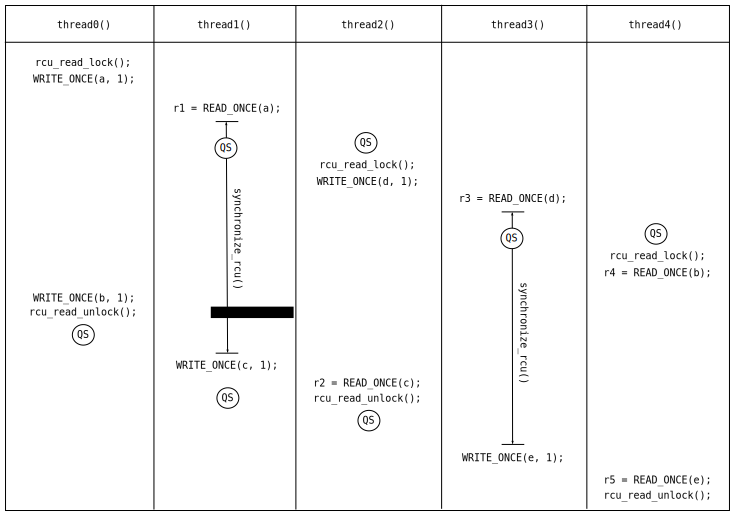
\includegraphics{rcu/design/ReadersPartitionGP1}}
\end{center}

Again, an RCU read-side critical section can overlap almost all of a
given grace period, just so long as it does not overlap the entire grace
period.
As a result, an RCU read-side critical section cannot partition
a pair of RCU grace periods.

\QuickQuiz{
  How long a sequence of grace periods, each separated by an RCU
  read-side critical section, would be required to partition the RCU
  read-side critical sections at the beginning and end of the chain?
}\QuickQuizAnswer{
  In theory, an infinite number. In practice, an unknown number that is
  sensitive to both implementation details and timing considerations.
  Therefore, even in practice, RCU users must abide by the theoretical
  rather than the practical answer.
}\QuickQuizEnd


\subsection{Parallelism Facts of Life}

These parallelism facts of life are by no means specific to RCU, but the
RCU implementation must abide by them.
They therefore bear repeating:

\begin{enumerate}
\item Any CPU or task may be delayed at any time, and any attempts to avoid
   these delays by disabling preemption, interrupts, or whatever are
   completely futile.
   This is most obvious in preemptible user-level
   environments and in virtualized environments (where a given guest
   OS's VCPUs can be preempted at any time by the underlying
   hypervisor), but can also happen in bare-metal environments due to
   ECC errors, NMIs, and other hardware events.
   Although a delay of more
   than about 20~seconds can result in splats, the RCU implementation is
   obligated to use algorithms that can tolerate extremely long delays,
   but where ``extremely long'' is not long enough to allow wrap-around
   when incrementing a 64-bit counter.
\item Both the compiler and the CPU can reorder memory accesses.
   Where it
   matters, RCU must use compiler directives and memory-barrier
   instructions to preserve ordering.
\item Conflicting writes to memory locations in any given cache line will
   result in expensive cache misses.
   Greater numbers of concurrent
   writes and more-frequent concurrent writes will result in more
   dramatic slowdowns.
   RCU is therefore obligated to use algorithms that
   have sufficient locality to avoid significant performance and
   scalability problems.
\item As a rough rule of thumb, only one CPU's worth of processing may be
   carried out under the protection of any given exclusive lock.
   RCU
   must therefore use scalable locking designs.
\item Counters are finite, especially on 32-bit systems.
   RCU's use of
   counters must therefore tolerate counter wrap, or be designed such
   that counter wrap would take way more time than a single system is
   likely to run.
   An uptime of ten years is quite possible, a runtime of
   a century much less so.
   As an example of the latter, RCU's
   dyntick-idle nesting counter allows 54~bits for interrupt nesting
   level (this counter is 64~bits even on a 32-bit system).
   Overflowing
   this counter requires $2^54$ half-interrupts on a given CPU
   without that CPU ever going idle.
   If a half-interrupt happened every
   microsecond, it would take 570 years of runtime to overflow this
   counter, which is currently believed to be an acceptably long time.
\item Linux systems can have thousands of CPUs running a single Linux
   kernel in a single shared-memory environment.
   RCU must therefore pay
   close attention to high-end scalability.
\end{enumerate}

This last parallelism fact of life means that RCU must pay special
attention to the preceding facts of life.
The idea that Linux might
scale to systems with thousands of CPUs would have been met with some
skepticism in the 1990s, but these requirements would have otherwise
have been unsurprising, even in the early 1990s.


\subsection{Quality-of-Implementation Requirements}

These sections list quality-of-implementation requirements.
Although an
RCU implementation that ignores these requirements could still be used,
it would likely be subject to limitations that would make it
inappropriate for industrial-strength production use.
Classes of
quality-of-implementation requirements are as follows:

\begin{enumerate}
\item Specialization
\item Performance and Scalability
\item Forward Progress
\item Composability
\item Corner Cases
\end{enumerate}

These classes is covered in the following sections.


\subsubsection{Specialization}

RCU is and always has been intended primarily for read-mostly
situations, which means that RCU's read-side primitives are optimized,
often at the expense of its update-side primitives.
Experience thus far
is captured by the following list of situations:

\begin{enumerate}
\item Read-mostly data, where stale and inconsistent data is not a problem:
   RCU works great!
\item Read-mostly data, where data must be consistent: RCU works well.
\item Read-write data, where data must be consistent: RCU \emph{might} work OK.
   Or not.
\item Write-mostly data, where data must be consistent: RCU is very
   unlikely to be the right tool for the job, with the following
   exceptions, where RCU can provide:

   \begin{enumerate}
   \item Existence guarantees for update-friendly mechanisms.
   \item Wait-free read-side primitives for real-time use.
   \end{enumerate}
\end{enumerate}

This focus on read-mostly situations means that RCU must interoperate
with other synchronization primitives.
For example, the \co{add_gp()} and
\co{remove_gp_synchronous()} examples discussed earlier use RCU to
protect readers and locking to coordinate updaters.
However, the need
extends much farther, requiring that a variety of synchronization
primitives be legal within RCU read-side critical sections, including
spinlocks, sequence locks, atomic operations, reference counters, and
memory barriers.

\QuickQuiz{
  What about sleeping locks?
}\QuickQuizAnswer{
  These are forbidden within Linux-kernel RCU read-side critical
  sections because it is not legal to place a quiescent state (in this
  case, voluntary context switch) within an RCU read-side critical
  section.
  However, sleeping locks may be used within userspace RCU
  read-side critical sections, and also within Linux-kernel sleepable
  RCU (SRCU) %`(SRCU) <Sleepable RCU_>`__
  read-side critical sections.
  In
  addition, the \co{-rt} patchset turns spinlocks into a sleeping locks so
  that the corresponding critical sections can be preempted, which also
  means that these sleeplockified spinlocks (but not other sleeping
  locks!) may be acquire within \co{-rt}-Linux-kernel RCU read-side critical
  sections.
  Note that it \emph{is} legal for a normal RCU read-side critical section
  to conditionally acquire a sleeping locks (as in
  \co{mutex_trylock()}), but only as long as it does not loop
  indefinitely attempting to conditionally acquire that sleeping locks.
  The key point is that things like \co{mutex_trylock()} either return
  with the mutex held, or return an error indication if the mutex was
  not immediately available. Either way, \co{mutex_trylock()} returns
  immediately without sleeping.
}\QuickQuizEnd

It often comes as a surprise that many algorithms do not require a
consistent view of data, but many can function in that mode, with
network routing being the poster child.
Internet routing algorithms take
significant time to propagate updates, so that by the time an update
arrives at a given system, that system has been sending network traffic
the wrong way for a considerable length of time.
Having a few threads
continue to send traffic the wrong way for a few more milliseconds is
clearly not a problem:
In the worst case, TCP retransmissions will
eventually get the data where it needs to go.
In general, when tracking
the state of the universe outside of the computer, some level of
inconsistency must be tolerated due to speed-of-light delays if nothing
else.

Furthermore, uncertainty about external state is inherent in many cases.
For example, a pair of veterinarians might use heartbeat to determine
whether or not a given cat was alive.
But how long should they wait
after the last heartbeat to decide that the cat is in fact dead?
Waiting
less than 400 milliseconds makes no sense because this would mean that a
relaxed cat would be considered to cycle between death and life more
than 100 times per minute.
Moreover, just as with human beings, a cat's
heart might stop for some period of time, so the exact wait period is a
judgment call.
One of our pair of veterinarians might wait 30 seconds
before pronouncing the cat dead, while the other might insist on waiting
a full minute.
The two veterinarians would then disagree on the state of
the cat during the final 30 seconds of the minute following the last
heartbeat.

Interestingly enough, this same situation applies to hardware.
When push
comes to shove, how do we tell whether or not some external server has
failed?
We send messages to it periodically, and declare it failed if we
don't receive a response within a given period of time.
Policy decisions
can usually tolerate short periods of inconsistency.
The policy was
decided some time ago, and is only now being put into effect, so a few
milliseconds of delay is normally inconsequential.

However, there are algorithms that absolutely must see consistent data.
For example, the translation between a user-level SystemV semaphore ID
to the corresponding in-kernel data structure is protected by RCU, but
it is absolutely forbidden to update a semaphore that has just been
removed.
In the Linux kernel, this need for consistency is accommodated
by acquiring spinlocks located in the in-kernel data structure from
within the RCU read-side critical section, and this is indicated by the
green box in the figure above. Many other techniques may be used, and
are in fact used within the Linux kernel.

In short, RCU is not required to maintain consistency, and other
mechanisms may be used in concert with RCU when consistency is required.
RCU's specialization allows it to do its job extremely well, and its
ability to interoperate with other synchronization mechanisms allows the
right mix of synchronization tools to be used for a given job.


\subsubsection{Performance and Scalability}

Energy efficiency is a critical component of performance today, and
Linux-kernel RCU implementations must therefore avoid unnecessarily
awakening idle CPUs.
I cannot claim that this requirement was
premeditated.
In fact, I learned of it during a telephone conversation
in which I was given ``frank and open'' feedback on the importance of
energy efficiency in battery-powered systems and on specific
energy-efficiency shortcomings of the Linux-kernel RCU implementation.
In my experience, the battery-powered embedded community will consider
any unnecessary wakeups to be extremely unfriendly acts.
So much so that
mere Linux-kernel-mailing-list posts are insufficient to vent their ire.

Memory consumption is not particularly important for in most situations,
and has become decreasingly so as memory sizes have expanded and memory
costs have plummeted.
However, as I learned from Matt Mackall's
\href{http://elinux.org/Linux_Tiny-FAQ}{bloatwatch} efforts, memory
footprint is critically important on single-CPU systems with
non-preemptible (\co{CONFIG_PREEMPTION=n}) kernels, and thus
\href{https://lore.kernel.org/r/20090113221724.GA15307@linux.vnet.ibm.com}{tiny RCU}
was born.
Josh Triplett has since taken over the small-memory banner
with his \href{https://tiny.wiki.kernel.org/}{Linux kernel tinification}
project, which resulted in SRCU %`SRCU <Sleepable RCU_>`__
becoming optional
for those kernels not needing it.

The remaining performance requirements are, for the most part,
unsurprising.
For example, in keeping with RCU's read-side
specialization, \co{rcu_dereference()} should have negligible overhead
(for example, suppression of a few minor compiler optimizations).
Similarly, in non-preemptible environments, \co{rcu_read_lock()} and
\co{rcu_read_unlock()} should have exactly zero overhead.

In preemptible environments, in the case where the RCU read-side
critical section was not preempted (as will be the case for the
highest-priority real-time process), \co{rcu_read_lock()} and
\co{rcu_read_unlock()} should have minimal overhead.
In particular, they
should not contain atomic read-modify-write operations, memory-barrier
instructions, preemption disabling, interrupt disabling, or backwards
branches.
However, in the case where the RCU read-side critical section
was preempted, \co{rcu_read_unlock()} may acquire spinlocks and disable
interrupts.
This is why it is better to nest an RCU read-side critical
section within a preempt-disable region than vice versa, at least in
cases where that critical section is short enough to avoid unduly
degrading real-time latencies.

The \co{synchronize_rcu()} grace-period-wait primitive is optimized for
throughput.
It may therefore incur several milliseconds of latency in
addition to the duration of the longest RCU read-side critical section.
On the other hand, multiple concurrent invocations of
\co{synchronize_rcu()} are required to use batching optimizations so that
they can be satisfied by a single underlying grace-period-wait
operation.
For example, in the Linux kernel, it is not unusual for a
single grace-period-wait operation to serve more than
\href{https://www.usenix.org/conference/2004-usenix-annual-technical-conference/making-rcu-safe-deep-sub-millisecond-response}{1,000 separate invocations}
of \co{synchronize_rcu()}, thus amortizing the per-invocation overhead
down to nearly zero.
However, the grace-period optimization is also
required to avoid measurable degradation of real-time scheduling and
interrupt latencies.

In some cases, the multi-millisecond \co{synchronize_rcu()} latencies are
unacceptable.
In these cases, \co{synchronize_rcu_expedited()} may be
used instead, reducing the grace-period latency down to a few tens of
microseconds on small systems, at least in cases where the RCU read-side
critical sections are short.
There are currently no special latency
requirements for \co{synchronize_rcu_expedited()} on large systems, but,
consistent with the empirical nature of the RCU specification, that is
subject to change.
However, there most definitely are scalability
requirements:
A storm of \co{synchronize_rcu_expedited()} invocations on
4096 CPUs should at least make reasonable forward progress.
In return
for its shorter latencies, \co{synchronize_rcu_expedited()} is permitted
to impose modest degradation of real-time latency on non-idle online
CPUs.
Here, ``modest'' means roughly the same latency degradation as a
scheduling-clock interrupt.

There are a number of situations where even
\co{synchronize_rcu_expedited()}'s reduced grace-period latency is
unacceptable.
In these situations, the \co{asynchronous call_rcu()} can
be used in place of \co{synchronize_rcu()} as follows:

\begin{VerbatimN}
       1 struct foo {
       2   int a;
       3   int b;
       4   struct rcu_head rh;
       5 };
       6
       7 static void remove_gp_cb(struct rcu_head *rhp)
       8 {
       9   struct foo *p = container_of(rhp, struct foo, rh);
      10
      11   kfree(p);
      12 }
      13
      14 bool remove_gp_asynchronous(void)
      15 {
      16   struct foo *p;
      17
      18   spin_lock(&gp_lock);
      19   p = rcu_access_pointer(gp);
      20   if (!p) {
      21     spin_unlock(&gp_lock);
      22     return false;
      23   }
      24   rcu_assign_pointer(gp, NULL);
      25   call_rcu(&p->rh, remove_gp_cb);
      26   spin_unlock(&gp_lock);
      27   return true;
      28 }
\end{VerbatimN}

A definition of \co{struct foo} is finally needed, and appears on
\clnrefrange{}{}. % lines 1-5
The function \co{remove_gp_cb()} is passed to \co{call_rcu()}
on \clnref{}, % line 25
and will be invoked after the end of a subsequent grace
period.
This gets the same effect as \co{remove_gp_synchronous()}, but
without forcing the updater to wait for a grace period to elapse.
The
\co{call_rcu()} function may be used in a number of situations where
neither \co{synchronize_rcu()} nor \co{synchronize_rcu_expedited()} would
be legal, including within preempt-disable code, \co{local_bh_disable()}
code, interrupt-disable code, and interrupt handlers.
However, even
\co{call_rcu()} is illegal within NMI handlers and from idle and offline
CPUs.
The callback function (\co{remove_gp_cb()} in this case) will be
executed within softirq (software interrupt) environment within the
Linux kernel, either within a real softirq handler or under the
protection of \co{local_bh_disable()}.
In both the Linux kernel and in
userspace, it is bad practice to write an RCU callback function that
takes too long.
Long-running operations should be relegated to separate
threads or (in the Linux kernel) workqueues.

\QuickQuiz{
  Why does \clnref{} % line 19
  use \co{rcu_access_pointer()}? After all,
  \co{call_rcu()} on \clnref{} % line 25
  stores into the structure, which would
  interact badly with concurrent insertions.
  Doesn't this mean that
  \co{rcu_dereference()} is required?
}\QuickQuizAnswer{
  Presumably the \co{->gp_lock} acquired on \clnref{} % line 18
  excludes any
  changes, including any insertions that \co{rcu_dereference()} would
  protect against.
  Therefore, any insertions will be delayed until
  after \co{->gp_lock} is released on \clnref{}, % line 25
  which in turn means that
  \co{rcu_access_pointer()} suffices.
}\QuickQuizEnd

However, all that \co{remove_gp_cb()} is doing is invoking \co{kfree()} on
the data element.
This is a common idiom, and is supported by
\co{kfree_rcu()}, which allows ``fire and forget'' operation as shown
below:

\begin{VerbatimN}
       1 struct foo {
       2   int a;
       3   int b;
       4   struct rcu_head rh;
       5 };
       6
       7 bool remove_gp_faf(void)
       8 {
       9   struct foo *p;
      10
      11   spin_lock(&gp_lock);
      12   p = rcu_dereference(gp);
      13   if (!p) {
      14     spin_unlock(&gp_lock);
      15     return false;
      16   }
      17   rcu_assign_pointer(gp, NULL);
      18   kfree_rcu(p, rh);
      19   spin_unlock(&gp_lock);
      20   return true;
      21 }
\end{VerbatimN}

Note that \co{remove_gp_faf()} simply invokes \co{kfree_rcu()} and
proceeds, without any need to pay any further attention to the
subsequent grace period and \co{kfree()}.
It is permissible to invoke
\co{kfree_rcu()} from the same environments as for \co{call_rcu()}.
Interestingly enough, DYNIX/ptx had the equivalents of \co{call_rcu()}
and \co{kfree_rcu()}, but not \co{synchronize_rcu()}.
This was due to the
fact that RCU was not heavily used within DYNIX/ptx, so the very few
places that needed something like \co{synchronize_rcu()} simply
open-coded it.

\QuickQuiz{
  Earlier it was claimed that \co{call_rcu()} and \co{kfree_rcu()}
  allowed updaters to avoid being blocked by readers.
  But how can that
  be correct, given that the invocation of the callback and the freeing
  of the memory (respectively) must still wait for a grace period to
  elapse?
}\QuickQuizAnswer{
  We could define things this way, but keep in mind that this sort of
  definition would say that updates in garbage-collected languages
  cannot complete until the next time the garbage collector runs, which
  does not seem at all reasonable.
  The key point is that in most cases,
  an updater using either \co{call_rcu()} or \co{kfree_rcu()} can proceed
  to the next update as soon as it has invoked \co{call_rcu()} or
  \co{kfree_rcu()}, without having to wait for a subsequent grace
  period.
}\QuickQuizEnd

But what if the updater must wait for the completion of code to be
executed after the end of the grace period, but has other tasks that can
be carried out in the meantime? The polling-style
\co{get_state_synchronize_rcu()} and \co{cond_synchronize_rcu()} functions
may be used for this purpose, as shown below:

\begin{VerbatimN}
       1 bool remove_gp_poll(void)
       2 {
       3   struct foo *p;
       4   unsigned long s;
       5
       6   spin_lock(&gp_lock);
       7   p = rcu_access_pointer(gp);
       8   if (!p) {
       9     spin_unlock(&gp_lock);
      10     return false;
      11   }
      12   rcu_assign_pointer(gp, NULL);
      13   spin_unlock(&gp_lock);
      14   s = get_state_synchronize_rcu();
      15   do_something_while_waiting();
      16   cond_synchronize_rcu(s);
      17   kfree(p);
      18   return true;
      19 }
\end{VerbatimN}

On \clnref{}, % line 14
\co{get_state_synchronize_rcu()} obtains a ``cookie'' from RCU,
then \clnref{} % line 15
carries out other tasks, and finally, \clnref{} % line 16
returns
immediately if a grace period has elapsed in the meantime, but otherwise
waits as required.
The need for \co{get_state_synchronize_rcu} and
\co{cond_synchronize_rcu()} has appeared quite recently, so it is too
early to tell whether they will stand the test of time.

RCU thus provides a range of tools to allow updaters to strike the
required tradeoff between latency, flexibility and CPU overhead.


\subsubsection{Forward Progress}

In theory, delaying grace-period completion and callback invocation is
harmless.
In practice, not only are memory sizes finite but also
callbacks sometimes do wakeups, and sufficiently deferred wakeups can be
difficult to distinguish from system hangs.
Therefore, RCU must provide
a number of mechanisms to promote forward progress.

These mechanisms are not foolproof, nor can they be. For one simple
example, an infinite loop in an RCU read-side critical section must by
definition prevent later grace periods from ever completing.
For a more
involved example, consider a 64-CPU system built with
\co{CONFIG_RCU_NOCB_CPU=y} and booted with \co{rcu_nocbs=1-63}, where
CPUs~1 through~63 spin in tight loops that invoke \co{call_rcu()}.
Even
if these tight loops also contain calls to \co{cond_resched()} (thus
allowing grace periods to complete), CPU~0 simply will not be able to
invoke callbacks as fast as the other 63 CPUs can register them, at
least not until the system runs out of memory.
In both of these
examples, the Spiderman principle applies:
With great power comes great
responsibility.
However, short of this level of abuse, RCU is required
to ensure timely completion of grace periods and timely invocation of
callbacks.

RCU takes the following steps to encourage timely completion of grace
periods:

\begin{enumerate}
\item If a grace period fails to complete within 100 milliseconds, RCU
   causes future invocations of \co{cond_resched()} on the holdout CPUs
   to provide an RCU quiescent state.
   RCU also causes those CPUs'
   \co{need_resched()} invocations to return \co{true}, but only after the
   corresponding CPU's next scheduling-clock.
\item CPUs mentioned in the \co{nohz_full} kernel boot parameter can run
   indefinitely in the kernel without scheduling-clock interrupts, which
   defeats the above \co{need_resched()} strategem.
   RCU will therefore
   invoke \co{resched_cpu()} on any \co{nohz_full} CPUs still holding out
   after 109 milliseconds.
\item In kernels built with \co{CONFIG_RCU_BOOST=y}, if a given task that
   has been preempted within an RCU read-side critical section is
   holding out for more than 500 milliseconds, RCU will resort to
   priority boosting.
\item If a CPU is still holding out 10 seconds into the grace period, RCU
   will invoke \co{resched_cpu()} on it regardless of its \co{nohz_full}
   state.
\end{enumerate}

The above values are defaults for systems running with \co{HZ=1000}.
They
will vary as the value of \co{HZ} varies, and can also be changed using
the relevant Kconfig options and kernel boot parameters.
RCU currently
does not do much sanity checking of these parameters, so please use
caution when changing them.
Note that these forward-progress measures
are provided only for RCU, not for SRCU %`SRCU <Sleepable RCU_>`__
or Task RCU\@. %`Tasks RCU`_.

RCU takes the following steps in \co{call_rcu()} to encourage timely
invocation of callbacks when any given non-\co{rcu_nocbs} CPU has
10,000 callbacks, or has 10,000 more callbacks than it had the last time
encouragement was provided:

\begin{enumerate}
\item Starts a grace period, if one is not already in progress.
\item Forces immediate checking for quiescent states, rather than waiting
   for three milliseconds to have elapsed since the beginning of the
   grace period.
\item Immediately tags the CPU's callbacks with their grace period
   completion numbers, rather than waiting for the \co{RCU_SOFTIRQ}
   handler to get around to it.
\item Lifts callback-execution batch limits, which speeds up callback
   invocation at the expense of degrading realtime response.
\end{enumerate}

Again, these are default values when running at \co{HZ=1000}, and can be
overridden.
Again, these forward-progress measures are provided only for
RCU, not for SRCU %`SRCU <Sleepable RCU_>`__
or Task RCU. %`Tasks RCU`_
Even for RCU, callback-invocation forward
progress for \co{rcu_nocbs} CPUs is much less well-developed, in part
because workloads benefiting from \co{rcu_nocbs} CPUs tend to invoke
\co{call_rcu()} relatively infrequently.
If workloads emerge that need
both \co{rcu_nocbs} CPUs and high \co{call_rcu()} invocation rates, then
additional forward-progress work will be required.


\subsubsection{Composability}

Composability has received much attention in recent years, perhaps in
part due to the collision of multicore hardware with object-oriented
techniques designed in single-threaded environments for single-threaded
use.
And in theory, RCU read-side critical sections may be composed, and
in fact may be nested arbitrarily deeply.
In practice, as with all
real-world implementations of composable constructs, there are
limitations.

Implementations of RCU for which \co{rcu_read_lock()} and
\co{rcu_read_unlock()} generate no code, such as Linux-kernel RCU when
\co{CONFIG_PREEMPTION=n}, can be nested arbitrarily deeply.
After all, there
is no overhead. Except that if all these instances of
\co{rcu_read_lock()} and \co{rcu_read_unlock()} are visible to the
compiler, compilation will eventually fail due to exhausting memory,
mass storage, or user patience, whichever comes first.
If the nesting is
not visible to the compiler, as is the case with mutually recursive
functions each in its own translation unit, stack overflow will result.
If the nesting takes the form of loops, perhaps in the guise of tail
recursion, either the control variable will overflow or (in the Linux
kernel) you will get an RCU CPU stall warning. Nevertheless, this class
of RCU implementations is one of the most composable constructs in
existence.

RCU implementations that explicitly track nesting depth are limited by
the nesting-depth counter.
For example, the Linux kernel's preemptible
RCU limits nesting to \co{INT_MAX}. This should suffice for almost all
practical purposes.
That said, a consecutive pair of RCU read-side
critical sections between which there is an operation that waits for a
grace period cannot be enclosed in another RCU read-side critical
section.
This is because it is not legal to wait for a grace period
within an RCU read-side critical section:
To do so would result either
in deadlock or in RCU implicitly splitting the enclosing RCU read-side
critical section, neither of which is conducive to a long-lived and
prosperous kernel.

It is worth noting that RCU is not alone in limiting composability. For
example, many transactional-memory implementations prohibit composing a
pair of transactions separated by an irrevocable operation (for example,
a network receive operation).
For another example, lock-based critical
sections can be composed surprisingly freely, but only if deadlock is
avoided.

In short, although RCU read-side critical sections are highly
composable, care is required in some situations, just as is the case for
any other composable synchronization mechanism.


\subsubsection{Corner Cases}

A given RCU workload might have an endless and intense stream of RCU
read-side critical sections, perhaps even so intense that there was
never a point in time during which there was not at least one RCU
read-side critical section in flight.
RCU cannot allow this situation to
block grace periods: As long as all the RCU read-side critical sections
are finite, grace periods must also be finite.

That said, preemptible RCU implementations could potentially result in
RCU read-side critical sections being preempted for long durations,
which has the effect of creating a long-duration RCU read-side critical
section.
This situation can arise only in heavily loaded systems, but
systems using real-time priorities are of course more vulnerable.
Therefore, RCU priority boosting is provided to help deal with this
case.
That said, the exact requirements on RCU priority boosting will
likely evolve as more experience accumulates.

Other workloads might have very high update rates.
Although one can
argue that such workloads should instead use something other than RCU,
the fact remains that RCU must handle such workloads gracefully.
This
requirement is another factor driving batching of grace periods, but it
is also the driving force behind the checks for large numbers of queued
RCU callbacks in the \co{call_rcu()} code path.
Finally, high update
rates should not delay RCU read-side critical sections, although some
small read-side delays can occur when using
\co{synchronize_rcu_expedited()}, courtesy of this function's use of
\co{smp_call_function_single()}.

Although all three of these corner cases were understood in the early
1990s, a simple user-level test consisting of \co{close(open(path))} in a
tight loop in the early 2000s suddenly provided a much deeper
appreciation of the high-update-rate corner case.
This test also
motivated addition of some RCU code to react to high update rates, for
example, if a given CPU finds itself with more than 10,000 RCU callbacks
queued, it will cause RCU to take evasive action by more aggressively
starting grace periods and more aggressively forcing completion of
grace-period processing.
This evasive action causes the grace period to
complete more quickly, but at the cost of restricting RCU's batching
optimizations, thus increasing the CPU overhead incurred by that grace
period.


\subsection{Software-Engineering Requirements}

Between Murphy's Law and ``To err is human'', it is necessary to guard
against mishaps and misuse:

\begin{enumerate}
\item It is all too easy to forget to use \co{rcu_read_lock()} everywhere
   that it is needed, so kernels built with \co{CONFIG_PROVE_RCU=y} will
   splat if \co{rcu_dereference()} is used outside of an RCU read-side
   critical section.
   Update-side code can use
   \co{rcu_dereference_protected()}, which takes a
   \href{https://lwn.net/Articles/371986/}{lockdep expression} to indicate what is
   providing the protection.
   If the indicated protection is not
   provided, a lockdep splat is emitted.
   Code shared between readers and updaters can use
   \co{rcu_dereference_check()}, which also takes a lockdep expression,
   and emits a lockdep splat if neither \co{rcu_read_lock()} nor the
   indicated protection is in place.
   In addition,
   \co{rcu_dereference_raw()} is used in those (hopefully rare) cases
   where the required protection cannot be easily described.
   Finally,
   \co{rcu_read_lock_held()} is provided to allow a function to verify
   that it has been invoked within an RCU read-side critical section.
   I
   was made aware of this set of requirements shortly after Thomas
   Gleixner audited a number of RCU uses.
\item A given function might wish to check for RCU-related preconditions
   upon entry, before using any other RCU API\@.
   The
   \co{rcu_lockdep_assert()} does this job, asserting the expression in
   kernels having lockdep enabled and doing nothing otherwise.
\item It is also easy to forget to use \co{rcu_assign_pointer()} and
   \co{rcu_dereference()}, perhaps (incorrectly) substituting a simple
   assignment.
   To catch this sort of error, a given RCU-protected
   pointer may be tagged with \co{__rcu}, after which \co{sparse} will
   complain about simple-assignment accesses to that pointer.
   Arnd
   Bergmann made me aware of this requirement, and also supplied the
   needed \href{https://lwn.net/Articles/376011/}{patch series}.
\item Kernels built with \co{CONFIG_DEBUG_OBJECTS_RCU_HEAD=y} will splat if
   a data element is passed to \co{call_rcu()} twice in a row, without a
   grace period in between.
   (This error is similar to a double free.)
   The corresponding \co{rcu_head} structures that are dynamically
   allocated are automatically tracked, but \co{rcu_head} structures
   allocated on the stack must be initialized with
   \co{init_rcu_head_on_stack()} and cleaned up with
   \co{destroy_rcu_head_on_stack()}.
   Similarly, statically allocated
   non-stack \co{rcu_head} structures must be initialized with
   \co{init_rcu_head()} and cleaned up with \co{destroy_rcu_head()}.
   Mathieu Desnoyers made me aware of this requirement, and also
   supplied the needed
   \href{https://lore.kernel.org/r/20100319013024.GA28456@Krystal}{patch}.
\item An infinite loop in an RCU read-side critical section will eventually
   trigger an RCU CPU stall warning splat, with the duration of
   ``eventually'' being controlled by the \co{RCU_CPU_STALL_TIMEOUT}
   \co{Kconfig} option, or, alternatively, by the
   \co{rcupdate.rcu_cpu_stall_timeout} boot/sysfs parameter.
   However, RCU
   is not obligated to produce this splat unless there is a grace period
   waiting on that particular RCU read-side critical section.

   Some extreme workloads might intentionally delay RCU grace periods,
   and systems running those workloads can be booted with
   \co{rcupdate.rcu_cpu_stall_suppress} to suppress the splats.
   This
   kernel parameter may also be set via \co{sysfs}. Furthermore, RCU CPU
   stall warnings are counter-productive during sysrq dumps and during
   panics.
   RCU therefore supplies the \co{rcu_sysrq_start()} and
   \co{rcu_sysrq_end()} API members to be called before and after long
   sysrq dumps.
   RCU also supplies the \co{rcu_panic()} notifier that is
   automatically invoked at the beginning of a panic to suppress further
   RCU CPU stall warnings.

   This requirement made itself known in the early 1990s, pretty much
   the first time that it was necessary to debug a CPU stall. That said,
   the initial implementation in DYNIX/ptx was quite generic in
   comparison with that of Linux.

\item Although it would be very good to detect pointers leaking out of RCU
   read-side critical sections, there is currently no good way of doing
   this.
   One complication is the need to distinguish between pointers
   leaking and pointers that have been handed off from RCU to some other
   synchronization mechanism, for example, reference counting.
\item In kernels built with \co{CONFIG_RCU_TRACE=y}, RCU-related information
   is provided via event tracing.
\item Open-coded use of \co{rcu_assign_pointer()} and \co{rcu_dereference()}
   to create typical linked data structures can be surprisingly
   error-prone. Therefore, RCU-protected
   \href{https://lwn.net/Articles/609973/#RCU%20List%20APIs}{linked lists} and,
   more recently, RCU-protected
   \href{https://lwn.net/Articles/612100/}{hash tables} are available.
   Many
   other special-purpose RCU-protected data structures are available in
   the Linux kernel and the userspace RCU library.
\item Some linked structures are created at compile time, but still require
   \co{__rcu} checking.
   The \co{RCU_POINTER_INITIALIZER()} macro serves
   this purpose.
\item It is not necessary to use \co{rcu_assign_pointer()} when creating
   linked structures that are to be published via a single external
   pointer.
   The \co{RCU_INIT_POINTER()} macro is provided for this task.
\end{enumerate}

This not a hard-and-fast list:
RCU's diagnostic capabilities will
continue to be guided by the number and type of usage bugs found in
real-world RCU usage.


\subsection{Linux Kernel Complications}

The Linux kernel provides an interesting environment for all kinds of
software, including RCU\@.
Some of the relevant points of interest are as
follows:

\begin{enumerate}
\item Configuration
\item Firmware Interface
\item Early Boot
\item Interrupts and NMIs
\item Loadable Modules
\item Hotplug CPU
\item Scheduler and RCU
\item Tracing and RCU
\item Accesses to User Memory and RCU
\item Energy Efficiency
\item Scheduling-Clock Interrupts and RCU
\item Memory Efficiency
\item Performance, Scalability, Response Time, and Reliability
\end{enumerate}

This list is probably incomplete, but it does give a feel for the most
notable Linux-kernel complications.
Each of the following sections
covers one of the above topics.


\subsubsection{Configuration}

RCU's goal is automatic configuration, so that almost nobody needs to
worry about RCU's \co{Kconfig} options.
And for almost all users, RCU
does in fact work well ``out of the box.''

However, there are specialized use cases that are handled by kernel boot
parameters and \co{Kconfig} options.
Unfortunately, the \co{Kconfig}
system will explicitly ask users about new \co{Kconfig} options, which
requires almost all of them be hidden behind a \co{CONFIG_RCU_EXPERT}
\co{Kconfig} option.

This all should be quite obvious, but the fact remains that Linus
Torvalds recently had to
\href{https://lore.kernel.org/r/CA+55aFy4wcCwaL4okTs8wXhGZ5h-ibecy_Meg9C4MNQrUnwMcg@mail.gmail.com>}{remind}
me of this requirement.


\subsubsection{Firmware Interface}

In many cases, kernel obtains information about the system from the
firmware, and sometimes things are lost in translation.
Or the
translation is accurate, but the original message is bogus.

For example, some systems' firmware overreports the number of CPUs,
sometimes by a large factor.
If RCU naively believed the firmware, as it
used to do, it would create too many per-CPU kthreads.
Although the
resulting system will still run correctly, the extra kthreads needlessly
consume memory and can cause confusion when they show up in \co{ps}
listings.

RCU must therefore wait for a given CPU to actually come online before
it can allow itself to believe that the CPU actually exists.
The
resulting ``ghost CPUs'' (which are never going to come online) cause a
number of \href{https://paulmck.livejournal.com/37494.html}{interesting complications}.


\subsubsection{Early Boot}

The Linux kernel's boot sequence is an interesting process, and RCU is
used early, even before \co{rcu_init()} is invoked.
In fact, a number of
RCU's primitives can be used as soon as the initial task's
\co{task_struct} is available and the boot CPU's per-CPU variables are
set up.
The read-side primitives (\co{rcu_read_lock()},
\co{rcu_read_unlock()}, \co{rcu_dereference()}, and
\co{rcu_access_pointer()}) will operate normally very early on, as will
\co{rcu_assign_pointer()}.

Although \co{call_rcu()} may be invoked at any time during boot,
callbacks are not guaranteed to be invoked until after all of RCU's
kthreads have been spawned, which occurs at \co{early_initcall()} time.
This delay in callback invocation is due to the fact that RCU does not
invoke callbacks until it is fully initialized, and this full
initialization cannot occur until after the scheduler has initialized
itself to the point where RCU can spawn and run its kthreads.
In theory,
it would be possible to invoke callbacks earlier, however, this is not a
panacea because there would be severe restrictions on what operations
those callbacks could invoke.

Perhaps surprisingly, \co{synchronize_rcu()} and
\co{synchronize_rcu_expedited()}, will operate normally during very early
boot, the reason being that there is only one CPU and preemption is
disabled.
This means that the call \co{synchronize_rcu()} (or friends)
itself is a quiescent state and thus a grace period, so the early-boot
implementation can be a no-op.

However, once the scheduler has spawned its first kthread, this early
boot trick fails for \co{synchronize_rcu()} (as well as for
\co{synchronize_rcu_expedited()}) in \co{CONFIG_PREEMPTION=y} kernels.
The
reason is that an RCU read-side critical section might be preempted,
which means that a subsequent \co{synchronize_rcu()} really does have to
wait for something, as opposed to simply returning immediately.
Unfortunately, \co{synchronize_rcu()} can't do this until all of its
kthreads are spawned, which doesn't happen until some time during
\co{early_initcalls()} time. But this is no excuse:
RCU is nevertheless
required to correctly handle synchronous grace periods during this time
period.
Once all of its kthreads are up and running, RCU starts running
normally.

\QuickQuiz{
  How can RCU possibly handle grace periods before all of its kthreads
  have been spawned???
}\QuickQuizAnswer{
  Very carefully!
  During the ``dead zone'' between the time that the scheduler spawns the
  first task and the time that all of RCU's kthreads have been spawned,
  all synchronous grace periods are handled by the expedited
  grace-period mechanism.
  At runtime, this expedited mechanism relies
  on workqueues, but during the dead zone the requesting task itself
  drives the desired expedited grace period.
  Because dead-zone
  execution takes place within task context, everything works.
  Once the
  dead zone ends, expedited grace periods go back to using workqueues,
  as is required to avoid problems that would otherwise occur when a
  user task received a POSIX signal while driving an expedited grace
  period.

  And yes, this does mean that it is unhelpful to send POSIX signals to
  random tasks between the time that the scheduler spawns its first
  kthread and the time that RCU's kthreads have all been spawned.
  If
  there ever turns out to be a good reason for sending POSIX signals
  during that time, appropriate adjustments will be made.
  (If it turns
  out that POSIX signals are sent during this time for no good reason,
  other adjustments will be made, appropriate or otherwise.)
}\QuickQuizEnd

I learned of these boot-time requirements as a result of a series of
system hangs.


\subsubsection{Interrupts and NMIs}

The Linux kernel has interrupts, and RCU read-side critical sections are
legal within interrupt handlers and within interrupt-disabled regions of
code, as are invocations of \co{call_rcu()}.

Some Linux-kernel architectures can enter an interrupt handler from
non-idle process context, and then just never leave it, instead
stealthily transitioning back to process context.
This trick is
sometimes used to invoke system calls from inside the kernel. These
``half-interrupts'' mean that RCU has to be very careful about how it
counts interrupt nesting levels.
I learned of this requirement the hard
way during a rewrite of RCU's dyntick-idle code.

The Linux kernel has non-maskable interrupts (NMIs), and RCU read-side
critical sections are legal within NMI handlers.
Thankfully, RCU
update-side primitives, including \co{call_rcu()}, are prohibited within
NMI handlers.

The name notwithstanding, some Linux-kernel architectures can have
nested NMIs, which RCU must handle correctly. Andy Lutomirski
\href{https://lore.kernel.org/r/CALCETrXLq1y7e_dKFPgou-FKHB6Pu-r8+t-6Ds+8=va7anBWDA@mail.gmail.com}{surprised me}
with this requirement; he also kindly surprised me with
\href{https://lore.kernel.org/r/CALCETrXSY9JpW3uE6H8WYk81sg56qasA2aqmjMPsq5dOtzso=g@mail.gmail.com}{an algorithm}
that meets this requirement.

Furthermore, NMI handlers can be interrupted by what appear to RCU to be
normal interrupts.
One way that this can happen is for code that
directly invokes \co{ct_irq_enter()} and \co{ct_irq_exit()} to be called
from an NMI handler.
This astonishing fact of life prompted the current
code structure, which has \co{ct_irq_enter()} invoking
\co{ct_nmi_enter()} and \co{ct_irq_exit()} invoking \co{ct_nmi_exit()}.
And yes, I also learned of this requirement the hard way.


\subsubsection{Loadable Modules}

The Linux kernel has loadable modules, and these modules can also be
unloaded.
After a given module has been unloaded, any attempt to call
one of its functions results in a segmentation fault.
The module-unload
functions must therefore cancel any delayed calls to loadable-module
functions, for example, any outstanding \co{mod_timer()} must be dealt
with via \co{timer_shutdown_sync()} or similar.

Unfortunately, there is no way to cancel an RCU callback; once you
invoke \co{call_rcu()}, the callback function is eventually going to be
invoked, unless the system goes down first.
Because it is normally
considered socially irresponsible to crash the system in response to a
module unload request, we need some other way to deal with in-flight RCU
callbacks.

RCU therefore provides \co{rcu_barrier()}, which waits until all
in-flight RCU callbacks have been invoked.
If a module uses
\co{call_rcu()}, its exit function should therefore prevent any future
invocation of \co{call_rcu()}, then invoke \co{rcu_barrier()}.
In theory,
the underlying module-unload code could invoke \co{rcu_barrier()}
unconditionally, but in practice this would incur unacceptable
latencies.

Nikita Danilov noted this requirement for an analogous
filesystem-unmount situation, and Dipankar Sarma incorporated
\co{rcu_barrier()} into RCU\@.
The need for \co{rcu_barrier()} for module
unloading became apparent later.

\begin{Note}
   important:

   The \co{rcu_barrier()} function is not, repeat,
   \emph{not}, obligated to wait for a grace period.
   It is instead only required
   to wait for RCU callbacks that have already been posted.
   Therefore, if
   there are no RCU callbacks posted anywhere in the system,
   \co{rcu_barrier()} is within its rights to return immediately.
   Even if
   there are callbacks posted, \co{rcu_barrier()} does not necessarily need
   to wait for a grace period.
\end{Note}

\QuickQuiz{
  Wait a minute!
  Each RCU callbacks must wait for a grace period to
  complete, and \co{rcu_barrier()} must wait for each pre-existing
  callback to be invoked.
  Doesn't \co{rcu_barrier()} therefore need to
  wait for a full grace period if there is even one callback posted
  anywhere in the system?
}\QuickQuizAnswer{
  Absolutely not!!!
  Yes, each RCU callbacks must wait for a grace period to complete, but
  it might well be partly (or even completely) finished waiting by the
  time \co{rcu_barrier()} is invoked.
  In that case, \co{rcu_barrier()}
  need only wait for the remaining portion of the grace period to
  elapse.
  So even if there are quite a few callbacks posted,
  \co{rcu_barrier()} might well return quite quickly.

  So if you need to wait for a grace period as well as for all
  pre-existing callbacks, you will need to invoke both
  \co{synchronize_rcu()} and \co{rcu_barrier()}.
  If latency is a concern,
  you can always use workqueues to invoke them concurrently.
}\QuickQuizEnd


\subsubsection{Hotplug CPU}

The Linux kernel supports CPU hotplug, which means that CPUs can come
and go.
It is of course illegal to use any RCU API member from an
offline CPU, with the exception of SRCU % `SRCU <Sleepable RCU_>`__
read-side
critical sections.
This requirement was present from day one in
DYNIX/ptx, but on the other hand, the Linux kernel's CPU-hotplug
implementation is ``interesting.''

The Linux-kernel CPU-hotplug implementation has notifiers that are used
to allow the various kernel subsystems (including RCU) to respond
appropriately to a given CPU-hotplug operation.
Most RCU operations may
be invoked from CPU-hotplug notifiers, including even synchronous
grace-period operations such as (\co{synchronize_rcu()} and
\co{synchronize_rcu_expedited()}).
However, these synchronous operations
do block and therefore cannot be invoked from notifiers that execute via
\co{stop_machine()}, specifically those between the \co{CPUHP_AP_OFFLINE}
and \co{CPUHP_AP_ONLINE} states.

In addition, all-callback-wait operations such as \co{rcu_barrier()} may
not be invoked from any CPU-hotplug notifier.
This restriction is due
to the fact that there are phases of CPU-hotplug operations where the
outgoing CPU's callbacks will not be invoked until after the CPU-hotplug
operation ends, which could also result in deadlock.
Furthermore,
\co{rcu_barrier()} blocks CPU-hotplug operations during its execution,
which results in another type of deadlock when invoked from a CPU-hotplug
notifier.

Finally, RCU must avoid deadlocks due to interaction between hotplug,
timers and grace period processing.
It does so by maintaining its own set
of books that duplicate the centrally maintained \co{cpu_online_mask},
and also by reporting quiescent states explicitly when a CPU goes
offline.
This explicit reporting of quiescent states avoids any need
for the force-quiescent-state loop (FQS) to report quiescent states for
offline CPUs.
However, as a debugging measure, the FQS loop does splat
if offline CPUs block an RCU grace period for too long.

An offline CPU's quiescent state will be reported either:

\begin{enumerate}
\item  As the CPU goes offline using RCU's hotplug notifier (\co{rcutree_report_cpu_dead()}).
\item  When grace period initialization (\co{rcu_gp_init()}) detects a
    race either with CPU offlining or with a task unblocking on a leaf
    \co{rcu_node} structure whose CPUs are all offline.
\end{enumerate}

The CPU-online path (\co{rcutree_report_cpu_starting()}) should never need to report
a quiescent state for an offline CPU\@.
However, as a debugging measure,
it does emit a warning if a quiescent state was not already reported
for that CPU\@.

During the checking/modification of RCU's hotplug bookkeeping, the
corresponding CPU's leaf node lock is held.
This avoids race conditions
between RCU's hotplug notifier hooks, the grace period initialization
code, and the FQS loop, all of which refer to or modify this bookkeeping.


\subsubsection{Scheduler and RCU}

RCU makes use of kthreads, and it is necessary to avoid excessive CPU-time
accumulation by these kthreads.
This requirement was no surprise, but
RCU's violation of it when running context-switch-heavy workloads when
built with \co{CONFIG_NO_HZ_FULL=y}
\href{http://www.rdrop.com/users/paulmck/scalability/paper/BareMetal.2015.01.15b.pdf}{did come as a surprise [PDF]}.
RCU has made good progress towards meeting this requirement, even for
context-switch-heavy \co{CONFIG_NO_HZ_FULL=y} workloads, but there is
room for further improvement.

There is no longer any prohibition against holding any of
scheduler's runqueue or priority-inheritance spinlocks across an
\co{rcu_read_unlock()}, even if interrupts and preemption were enabled
somewhere within the corresponding RCU read-side critical section.
Therefore, it is now perfectly legal to execute \co{rcu_read_lock()}
with preemption enabled, acquire one of the scheduler locks, and hold
that lock across the matching \co{rcu_read_unlock()}.

Similarly, the RCU flavor consolidation has removed the need for negative
nesting.
The fact that interrupt-disabled regions of code act as RCU
read-side critical sections implicitly avoids earlier issues that used
to result in destructive recursion via interrupt handler's use of RCU\@.


\subsubsection{Tracing and RCU}

It is possible to use tracing on RCU code, but tracing itself uses RCU\@.
For this reason, \co{rcu_dereference_raw_check()} is provided for use
by tracing, which avoids the destructive recursion that could otherwise
ensue.
This API is also used by virtualization in some architectures,
where RCU readers execute in environments in which tracing cannot be
used.
The tracing folks both located the requirement and provided the
needed fix, so this surprise requirement was relatively painless.


\subsubsection{Accesses to User Memory and RCU}

The kernel needs to access user-space memory, for example, to access data
referenced by system-call parameters.
The \co{get_user()} macro does this job.

However, user-space memory might well be paged out, which means that
\co{get_user()} might well page-fault and thus block while waiting for the
resulting I/O to complete.
It would be a very bad thing for the compiler to
reorder a \co{get_user()} invocation into an RCU read-side critical section.

For example, suppose that the source code looked like this:

\begin{VerbatimN}
       1 rcu_read_lock();
       2 p = rcu_dereference(gp);
       3 v = p->value;
       4 rcu_read_unlock();
       5 get_user(user_v, user_p);
       6 do_something_with(v, user_v);
\end{VerbatimN}

The compiler must not be permitted to transform this source code into
the following:

\begin{VerbatimN}
       1 rcu_read_lock();
       2 p = rcu_dereference(gp);
       3 get_user(user_v, user_p); // BUG: POSSIBLE PAGE FAULT!!!
       4 v = p->value;
       5 rcu_read_unlock();
       6 do_something_with(v, user_v);
\end{VerbatimN}

If the compiler did make this transformation in a \co{CONFIG_PREEMPTION=n} kernel
build, and if \co{get_user()} did page fault, the result would be a quiescent
state in the middle of an RCU read-side critical section.
This misplaced
quiescent state could result in \clnref{} % line 4
being a use-after-free access,
which could be bad for your kernel's actuarial statistics.
Similar examples
can be constructed with the call to \co{get_user()} preceding the
\co{rcu_read_lock()}.

Unfortunately, \co{get_user()} doesn't have any particular ordering properties,
and in some architectures the underlying \co{asm} isn't even marked
\co{volatile}.
And even if it was marked \co{volatile}, the above access to
\co{p->value} is not volatile, so the compiler would not have any reason to keep
those two accesses in order.

Therefore, the Linux-kernel definitions of \co{rcu_read_lock()} and
\co{rcu_read_unlock()} must act as compiler barriers, at least for outermost
instances of \co{rcu_read_lock()} and \co{rcu_read_unlock()} within a nested set
of RCU read-side critical sections.


\subsubsection{Energy Efficiency}

Interrupting idle CPUs is considered socially unacceptable, especially
by people with battery-powered embedded systems.
RCU therefore conserves
energy by detecting which CPUs are idle, including tracking CPUs that
have been interrupted from idle.
This is a large part of the
energy-efficiency requirement, so I learned of this via an irate phone
call.

Because RCU avoids interrupting idle CPUs, it is illegal to execute an
RCU read-side critical section on an idle CPU.
(Kernels built with
\co{CONFIG_PROVE_RCU=y} will splat if you try it.)

It is similarly socially unacceptable to interrupt an \co{nohz_full} CPU
running in userspace.
RCU must therefore track \co{nohz_full} userspace
execution.
RCU must therefore be able to sample state at two points in
time, and be able to determine whether or not some other CPU spent any
time idle and/or executing in userspace.

These energy-efficiency requirements have proven quite difficult to
understand and to meet, for example, there have been more than five
clean-sheet rewrites of RCU's energy-efficiency code, the last of which
was finally able to demonstrate
\href{http://www.rdrop.com/users/paulmck/realtime/paper/AMPenergy.2013.04.19a.pdf}{real energy savings running on real hardware [PDF]}.
As noted earlier, I learned of many of these requirements via angry
phone calls:
Flaming me on the Linux-kernel mailing list was apparently
not sufficient to fully vent their ire at RCU's energy-efficiency bugs!


\subsubsection{Scheduling-Clock Interrupts and RCU}

The kernel transitions between in-kernel non-idle execution, userspace
execution, and the idle loop.
Depending on kernel configuration, RCU
handles these states differently:

\begin{VerbatimU}
+-------------+------------------+------------------+-----------------+
| HZ Kconfig  | In-Kernel        | Usermode         | Idle            |
+=============+==================+==================+=================+
| HZ_PERIODIC | Can rely on      | Can rely on      | Can rely on     |
|             | scheduling-clock | scheduling-clock | RCU's           |
|             | interrupt.       | interrupt and    | dyntick-idle    |
|             |                  | its detection    | detection.      |
|             |                  | of interrupt     |                 |
|             |                  | from usermode.   |                 |
+-------------+------------------+------------------+-----------------+
| NO_HZ_IDLE  | Can rely on      | Can rely on      | Can rely on     |
|             | scheduling-clock | scheduling-clock | RCU's           |
|             | interrupt.       | interrupt and    | dyntick-idle    |
|             |                  | its detection    | detection.      |
|             |                  | of interrupt     |                 |
|             |                  | from usermode.   |                 |
+-------------+------------------+------------------+-----------------+
| NO_HZ_FULL  | Can only         | Can rely on      | Can rely on     |
|             | sometimes rely   | RCU's            | RCU's           |
|             | on               | dyntick-idle     | dyntick-idle    |
|             | scheduling-clock | detection.       | detection.      |
|             | interrupt. In    |                  |                 |
|             | other cases, it  |                  |                 |
|             | is necessary to  |                  |                 |
|             | bound kernel     |                  |                 |
|             | execution times  |                  |                 |
|             | and/or use       |                  |                 |
|             | IPIs.            |                  |                 |
+-------------+------------------+------------------+-----------------+
\end{VerbatimU}

\QuickQuiz{
  Why can't \co{NO_HZ_FULL} in-kernel execution rely on the
  scheduling-clock interrupt, just like \co{HZ_PERIODIC} and
  \co{NO_HZ_IDLE} do?
}\QuickQuizAnswer{
  Because, as a performance optimization, \co{NO_HZ_FULL} does not
  necessarily re-enable the scheduling-clock interrupt on entry to each
  and every system call.
}\QuickQuizEnd

However, RCU must be reliably informed as to whether any given CPU is
currently in the idle loop, and, for \co{NO_HZ_FULL}, also whether that
CPU is executing in usermode, as discussed earlier. % `earlier <Energy Efficiency_>`__.
It also requires that the
scheduling-clock interrupt be enabled when RCU needs it to be:

\begin{enumerate}
\item If a CPU is either idle or executing in usermode, and RCU believes it
   is non-idle, the scheduling-clock tick had better be running.
   Otherwise, you will get RCU CPU stall warnings.
   Or at best, very long
   (11-second) grace periods, with a pointless IPI waking the CPU from
   time to time.
\item If a CPU is in a portion of the kernel that executes RCU read-side
   critical sections, and RCU believes this CPU to be idle, you will get
   random memory corruption.
   \textbf{DON'T DO THIS!!!}
   This is one reason to test with lockdep, which will complain about
   this sort of thing.
\item If a CPU is in a portion of the kernel that is absolutely positively
   no-joking guaranteed to never execute any RCU read-side critical
   sections, and RCU believes this CPU to be idle, no problem.
   This
   sort of thing is used by some architectures for light-weight
   exception handlers, which can then avoid the overhead of
   \co{ct_irq_enter()} and \co{ct_irq_exit()} at exception entry and
   exit, respectively.
   Some go further and avoid the entireties of
   \co{irq_enter()} and \co{irq_exit()}.
   Just make very sure you are running some of your tests with
   \co{CONFIG_PROVE_RCU=y}, just in case one of your code paths was in
   fact joking about not doing RCU read-side critical sections.
\item If a CPU is executing in the kernel with the scheduling-clock
   interrupt disabled and RCU believes this CPU to be non-idle, and if
   the CPU goes idle (from an RCU perspective) every few jiffies, no
   problem.
   It is usually OK for there to be the occasional gap between
   idle periods of up to a second or so.
   If the gap grows too long, you get RCU CPU stall warnings.
\item If a CPU is either idle or executing in usermode, and RCU believes it
   to be idle, of course no problem.
\item If a CPU is executing in the kernel, the kernel code path is passing
   through quiescent states at a reasonable frequency (preferably about
   once per few jiffies, but the occasional excursion to a second or so
   is usually OK) and the scheduling-clock interrupt is enabled, of
   course no problem.
   If the gap between a successive pair of quiescent states grows too
   long, you get RCU CPU stall warnings.
\end{enumerate}

\QuickQuiz{
  But what if my driver has a hardware interrupt handler that can run
  for many seconds?
  I cannot invoke \co{schedule()} from an hardware
  interrupt handler, after all!
}\QuickQuizAnswer{
  One approach is to do \co{ct_irq_exit(); ct_irq_enter();} every so
  often.
  But given that long-running interrupt handlers can cause other
  problems, not least for response time, shouldn't you work to keep
  your interrupt handler's runtime within reasonable bounds?
}\QuickQuizEnd

But as long as RCU is properly informed of kernel state transitions
between in-kernel execution, usermode execution, and idle, and as long
as the scheduling-clock interrupt is enabled when RCU needs it to be,
you can rest assured that the bugs you encounter will be in some other
part of RCU or some other part of the kernel!


\subsubsection{Memory Efficiency}

Although small-memory non-realtime systems can simply use Tiny RCU, code
size is only one aspect of memory efficiency.
Another aspect is the size
of the \co{rcu_head} structure used by \co{call_rcu()} and
\co{kfree_rcu()}.
Although this structure contains nothing more than a
pair of pointers, it does appear in many RCU-protected data structures,
including some that are size critical.
The \co{page} structure is a case
in point, as evidenced by the many occurrences of the \co{union} keyword
within that structure.

This need for memory efficiency is one reason that RCU uses hand-crafted
singly linked lists to track the \co{rcu_head} structures that are
waiting for a grace period to elapse.
It is also the reason why
\co{rcu_head} structures do not contain debug information, such as fields
tracking the file and line of the \co{call_rcu()} or \co{kfree_rcu()} that
posted them.
Although this information might appear in debug-only kernel
builds at some point, in the meantime, the \co{->func} field will often
provide the needed debug information.

However, in some cases, the need for memory efficiency leads to even
more extreme measures.
Returning to the \co{page} structure, the
\co{rcu_head} field shares storage with a great many other structures
that are used at various points in the corresponding page's lifetime.
In
order to correctly resolve certain
\href{https://lore.kernel.org/r/1439976106-137226-1-git-send-email-kirill.shutemov@linux.intel.com}{race conditions},
the Linux kernel's memory-management subsystem needs a particular bit to
remain zero during all phases of grace-period processing, and that bit
happens to map to the bottom bit of the \co{rcu_head} structure's
\co{->next} field.
RCU makes this guarantee as long as \co{call_rcu()} is
used to post the callback, as opposed to \co{kfree_rcu()} or some future
``lazy'' variant of \co{call_rcu()} that might one day be created for
energy-efficiency purposes.

That said, there are limits.
RCU requires that the \co{rcu_head}
structure be aligned to a two-byte boundary, and passing a misaligned
\co{rcu_head} structure to one of the \co{call_rcu()} family of functions
will result in a splat.
It is therefore necessary to exercise caution
when packing structures containing fields of type \co{rcu_head}.
Why not
a four-byte or even eight-byte alignment requirement?
Because the m68k
architecture provides only two-byte alignment, and thus acts as
alignment's least common denominator.

The reason for reserving the bottom bit of pointers to \co{rcu_head}
structures is to leave the door open to ``lazy'' callbacks whose
invocations can safely be deferred. Deferring invocation could
potentially have energy-efficiency benefits, but only if the rate of
non-lazy callbacks decreases significantly for some important workload.
In the meantime, reserving the bottom bit keeps this option open in case
it one day becomes useful.


\subsubsection{Performance, Scalability, Response Time, and Reliability}

Expanding on the earlier discussion, % `earlier discussion <Performance and Scalability_>`__
RCU is used heavily by
hot code paths in performance-critical portions of the Linux kernel's
networking, security, virtualization, and scheduling code paths.
RCU
must therefore use efficient implementations, especially in its
read-side primitives.
To that end, it would be good if preemptible RCU's
implementation of \co{rcu_read_lock()} could be inlined, however, doing
this requires resolving \co{#include} issues with the \co{task_struct}
structure.

The Linux kernel supports hardware configurations with up to 4096 CPUs,
which means that RCU must be extremely scalable.
Algorithms that involve
frequent acquisitions of global locks or frequent atomic operations on
global variables simply cannot be tolerated within the RCU
implementation. RCU therefore makes heavy use of a combining tree based
on the \co{rcu_node} structure.
RCU is required to tolerate all CPUs
continuously invoking any combination of RCU's runtime primitives with
minimal per-operation overhead.
In fact, in many cases, increasing load
must \emph{decrease} the per-operation overhead, witness the batching
optimizations for \co{synchronize_rcu()}, \co{call_rcu()},
\co{synchronize_rcu_expedited()}, and \co{rcu_barrier()}.
As a general
rule, RCU must cheerfully accept whatever the rest of the Linux kernel
decides to throw at it.

The Linux kernel is used for real-time workloads, especially in
conjunction with the
\href{https://wiki.linuxfoundation.org/realtime/}{\co{-rt} patchset}.
The
real-time-latency response requirements are such that the traditional
approach of disabling preemption across RCU read-side critical sections
is inappropriate.
Kernels built with \co{CONFIG_PREEMPTION=y} therefore use
an RCU implementation that allows RCU read-side critical sections to be
preempted.
This requirement made its presence known after users made it
clear that an earlier
\href{https://lwn.net/Articles/107930/}{real-time patch}
did not meet their needs, in
conjunction with some
\href{https://lore.kernel.org/r/20050318002026.GA2693@us.ibm.com}{RCU issues}
encountered by a very early version of the \co{-rt} patchset.

In addition, RCU must make do with a sub-100-microsecond real-time
latency budget.
In fact, on smaller systems with the \co{-rt} patchset, the
Linux kernel provides sub-20-microsecond real-time latencies for the
whole kernel, including RCU\@.
RCU's scalability and latency must
therefore be sufficient for these sorts of configurations.
To my
surprise, the sub-100-microsecond real-time latency budget
\href{http://www.rdrop.com/users/paulmck/realtime/paper/bigrt.2013.01.31a.LCA.pdf}{applies to even the largest systems [PDF]},
up to and including systems with 4096 CPUs.
This real-time requirement
motivated the grace-period kthread, which also simplified handling of a
number of race conditions.

RCU must avoid degrading real-time response for CPU-bound threads,
whether executing in usermode (which is one use case for
\co{CONFIG_NO_HZ_FULL=y}) or in the kernel.
That said, CPU-bound loops in
the kernel must execute \co{cond_resched()} at least once per few tens of
milliseconds in order to avoid receiving an IPI from RCU\@.

Finally, RCU's status as a synchronization primitive means that any RCU
failure can result in arbitrary memory corruption that can be extremely
difficult to debug.
This means that RCU must be extremely reliable,
which in practice also means that RCU must have an aggressive
stress-test suite.
This stress-test suite is called \co{rcutorture}.

Although the need for \co{rcutorture} was no surprise, the current
immense popularity of the Linux kernel is posing interesting---and perhaps
unprecedented---validation challenges.
To see this, keep in mind that
there are well over one billion instances of the Linux kernel running
today, given Android smartphones, Linux-powered televisions, and
servers.
This number can be expected to increase sharply with the advent
of the celebrated Internet of Things.

Suppose that RCU contains a race condition that manifests on average
once per million years of runtime.
This bug will be occurring about
three times per \emph{day} across the installed base. RCU could simply hide
behind hardware error rates, given that no one should really expect
their smartphone to last for a million years.
However, anyone taking too
much comfort from this thought should consider the fact that in most
jurisdictions, a successful multi-year test of a given mechanism, which
might include a Linux kernel, suffices for a number of types of
safety-critical certifications.
In fact, rumor has it that the Linux
kernel is already being used in production for safety-critical
applications.
I don't know about you, but I would feel quite bad if a
bug in RCU killed someone.
Which might explain my recent focus on
validation and verification.


\subsection{Other RCU Flavors}

One of the more surprising things about RCU is that there are now no
fewer than five \emph{flavors}, or API families.
In addition, the primary
flavor that has been the sole focus up to this point has two different
implementations, non-preemptible and preemptible.
The other four flavors
are listed below, with requirements for each described in a separate
section.

\begin{enumerate}
\item Bottom-Half Flavor (Historical)
\item Sched Flavor (Historical)
\item Sleepable RCU
\item Tasks RCU
\item Tasks Trace RCU
\end{enumerate}


\subsubsection{Bottom-Half Flavor (Historical)}

The RCU-bh flavor of RCU has since been expressed in terms of the other
RCU flavors as part of a consolidation of the three flavors into a
single flavor.
The read-side API remains, and continues to disable
softirq and to be accounted for by lockdep.
Much of the material in this
section is therefore strictly historical in nature.

The softirq-disable (AKA ``bottom-half'', hence the \qco{_bh} abbreviations)
flavor of RCU, or \emph{RCU-bh}, was developed by Dipankar Sarma to provide a
flavor of RCU that could withstand the network-based denial-of-service
attacks researched by Robert Olsson.
These attacks placed so much
networking load on the system that some of the CPUs never exited softirq
execution, which in turn prevented those CPUs from ever executing a
context switch, which, in the RCU implementation of that time, prevented
grace periods from ever ending.
The result was an out-of-memory
condition and a system hang.

The solution was the creation of RCU-bh, which does
\co{local_bh_disable()} across its read-side critical sections, and which
uses the transition from one type of softirq processing to another as a
quiescent state in addition to context switch, idle, user mode, and
offline.
This means that RCU-bh grace periods can complete even when
some of the CPUs execute in softirq indefinitely, thus allowing
algorithms based on RCU-bh to withstand network-based denial-of-service
attacks.

Because \co{rcu_read_lock_bh()} and \co{rcu_read_unlock_bh()} disable and
re-enable softirq handlers, any attempt to start a softirq handlers
during the RCU-bh read-side critical section will be deferred.
In this
case, \co{rcu_read_unlock_bh()} will invoke softirq processing, which can
take considerable time.
One can of course argue that this softirq
overhead should be associated with the code following the RCU-bh
read-side critical section rather than \co{rcu_read_unlock_bh()}, but the
fact is that most profiling tools cannot be expected to make this sort
of fine distinction.
For example, suppose that a three-millisecond-long
RCU-bh read-side critical section executes during a time of heavy
networking load.
There will very likely be an attempt to invoke at least
one softirq handler during that three milliseconds, but any such
invocation will be delayed until the time of the
\co{rcu_read_unlock_bh()}.
This can of course make it appear at first
glance as if \co{rcu_read_unlock_bh()} was executing very slowly.

The \href{https://lwn.net/Articles/609973/#RCU%20Per-Flavor%20API%20Table}{RCU-bh API}
includes \co{rcu_read_lock_bh()}, \co{rcu_read_unlock_bh()}, \co{rcu_dereference_bh()},
\co{rcu_dereference_bh_check()}, and \co{rcu_read_lock_bh_held()}.
However, the
old RCU-bh update-side APIs are now gone, replaced by \co{synchronize_rcu()},
\co{synchronize_rcu_expedited()}, \co{call_rcu()}, and \co{rcu_barrier()}.
In addition,
anything that disables bottom halves also marks an RCU-bh read-side
critical section, including \co{local_bh_disable()} and \co{local_bh_enable()},
\co{local_irq_save()} and \co{local_irq_restore()}, and so on.


\subsubsection{Sched Flavor (Historical)}

The RCU-sched flavor of RCU has since been expressed in terms of the
other RCU flavors as part of a consolidation of the three flavors into a
single flavor.
The read-side API remains, and continues to disable
preemption and to be accounted for by lockdep.
Much of the material in
this section is therefore strictly historical in nature.

Before preemptible RCU, waiting for an RCU grace period had the side
effect of also waiting for all pre-existing interrupt and NMI handlers.
However, there are legitimate preemptible-RCU implementations that do
not have this property, given that any point in the code outside of an
RCU read-side critical section can be a quiescent state.
Therefore,
\emph{RCU-sched} was created, which follows ``classic'' RCU in that an
RCU-sched grace period waits for pre-existing interrupt and NMI
handlers.
In kernels built with \co{CONFIG_PREEMPTION=n}, the RCU and
RCU-sched APIs have identical implementations, while kernels built with
\co{CONFIG_PREEMPTION=y} provide a separate implementation for each.

Note well that in \co{CONFIG_PREEMPTION=y} kernels,
\co{rcu_read_lock_sched()} and \co{rcu_read_unlock_sched()} disable and
re-enable preemption, respectively.
This means that if there was a
preemption attempt during the RCU-sched read-side critical section,
\co{rcu_read_unlock_sched()} will enter the scheduler, with all the
latency and overhead entailed.
Just as with \co{rcu_read_unlock_bh()},
this can make it look as if \co{rcu_read_unlock_sched()} was executing
very slowly. However, the highest-priority task won't be preempted, so
that task will enjoy low-overhead \co{rcu_read_unlock_sched()}
invocations.

The \href{https://lwn.net/Articles/609973/#RCU%20Per-Flavor%20API%20Table}{RCU-sched API}
includes \co{rcu_read_lock_sched()}, \co{rcu_read_unlock_sched()},
\co{rcu_read_lock_sched_notrace()}, \co{rcu_read_unlock_sched_notrace()},
\co{rcu_dereference_sched()}, \co{rcu_dereference_sched_check()}, and
\co{rcu_read_lock_sched_held()}.
However, the old RCU-sched update-side APIs
are now gone, replaced by \co{synchronize_rcu()}, \co{synchronize_rcu_expedited()},
\co{call_rcu()}, and \co{rcu_barrier()}.
In addition, anything that disables
preemption also marks an RCU-sched read-side critical section,
including \co{preempt_disable()} and \co{preempt_enable()}, \co{local_irq_save()}
and \co{local_irq_restore()}, and so on.


\subsubsection{Sleepable RCU}

For well over a decade, someone saying ``I need to block within an RCU
read-side critical section'' was a reliable indication that this someone
did not understand RCU\@.
After all, if you are always blocking in an RCU
read-side critical section, you can probably afford to use a
higher-overhead synchronization mechanism.
However, that changed with
the advent of the Linux kernel's notifiers, whose RCU read-side critical
sections almost never sleep, but sometimes need to.
This resulted in the
introduction of \href{https://lwn.net/Articles/202847/}{sleepable RCU}, or
\emph{SRCU}.

SRCU allows different domains to be defined, with each such domain
defined by an instance of an \co{srcu_struct} structure.
A pointer to
this structure must be passed in to each SRCU function, for example,
\co{synchronize_srcu(&ss)}, where \co{ss} is the \co{srcu_struct}
structure.
The key benefit of these domains is that a slow SRCU reader
in one domain does not delay an SRCU grace period in some other domain.
That said, one consequence of these domains is that read-side code must
pass a ``cookie'' from \co{srcu_read_lock()} to \co{srcu_read_unlock()}, for
example, as follows:

\begin{VerbatimN}
       1 int idx;
       2
       3 idx = srcu_read_lock(&ss);
       4 do_something();
       5 srcu_read_unlock(&ss, idx);
\end{VerbatimN}

As noted above, it is legal to block within SRCU read-side critical
sections, however, with great power comes great responsibility.
If you
block forever in one of a given domain's SRCU read-side critical
sections, then that domain's grace periods will also be blocked forever.
Of course, one good way to block forever is to deadlock, which can
happen if any operation in a given domain's SRCU read-side critical
section can wait, either directly or indirectly, for that domain's grace
period to elapse.
For example, this results in a self-deadlock:

\begin{VerbatimN}
       1 int idx;
       2
       3 idx = srcu_read_lock(&ss);
       4 do_something();
       5 synchronize_srcu(&ss);
       6 srcu_read_unlock(&ss, idx);
\end{VerbatimN}

However, if \clnref{} % line 5
acquired a mutex that was held across a
\co{synchronize_srcu()} for domain \co{ss}, deadlock would still be
possible.
Furthermore, if \clnref{} % line 5
acquired a mutex that was held across a
\co{synchronize_srcu()} for some other domain \co{ss1}, and if an
\co{ss1}-domain SRCU read-side critical section acquired another mutex
that was held across as \co{ss}-domain \co{synchronize_srcu()}, deadlock
would again be possible.
Such a deadlock cycle could extend across an
arbitrarily large number of different SRCU domains.
Again, with great
power comes great responsibility.

Unlike the other RCU flavors, SRCU read-side critical sections can run
on idle and even offline CPUs.
This ability requires that
\co{srcu_read_lock()} and \co{srcu_read_unlock()} contain memory barriers,
which means that SRCU readers will run a bit slower than would RCU
readers.
It also motivates the \co{smp_mb__after_srcu_read_unlock()} API,
which, in combination with \co{srcu_read_unlock()}, guarantees a full
memory barrier.

Also unlike other RCU flavors, \co{synchronize_srcu()} may \emph{not} be
invoked from CPU-hotplug notifiers, due to the fact that SRCU grace
periods make use of timers and the possibility of timers being
temporarily ``stranded'' on the outgoing CPU\@.
This stranding of timers
means that timers posted to the outgoing CPU will not fire until late in
the CPU-hotplug process.
The problem is that if a notifier is waiting on
an SRCU grace period, that grace period is waiting on a timer, and that
timer is stranded on the outgoing CPU, then the notifier will never be
awakened, in other words, deadlock has occurred.
This same situation of
course also prohibits \co{srcu_barrier()} from being invoked from
CPU-hotplug notifiers.

SRCU also differs from other RCU flavors in that SRCU's expedited and
non-expedited grace periods are implemented by the same mechanism.
This
means that in the current SRCU implementation, expediting a future grace
period has the side effect of expediting all prior grace periods that
have not yet completed.
(But please note that this is a property of the
current implementation, not necessarily of future implementations.)
In
addition, if SRCU has been idle for longer than the interval specified
by the \co{srcutree.exp_holdoff} kernel boot parameter (25 microseconds
by default), and if a \co{synchronize_srcu()} invocation ends this idle
period, that invocation will be automatically expedited.

As of v4.12, SRCU's callbacks are maintained per-CPU, eliminating a
locking bottleneck present in prior kernel versions.
Although this will
allow users to put much heavier stress on \co{call_srcu()}, it is
important to note that SRCU does not yet take any special steps to deal
with callback flooding. So if you are posting (say) 10,000 SRCU
callbacks per second per CPU, you are probably totally OK, but if you
intend to post (say) 1,000,000 SRCU callbacks per second per CPU, please
run some tests first.
SRCU just might need a few adjustment to deal with
that sort of load.
Of course, your mileage may vary based on the speed
of your CPUs and the size of your memory.

The \href{https://lwn.net/Articles/609973/#RCU%20Per-Flavor%20API%20Table}{SRCU API}
includes \co{srcu_read_lock()}, \co{srcu_read_unlock()},
\co{srcu_dereference()}, \co{srcu_dereference_check()},
\co{synchronize_srcu()}, \co{synchronize_srcu_expedited()},
\co{call_srcu()}, \co{srcu_barrier()}, and \co{srcu_read_lock_held()}.
It
also includes \co{DEFINE_SRCU()}, \co{DEFINE_STATIC_SRCU()}, and
\co{init_srcu_struct()} APIs for defining and initializing
\co{srcu_struct} structures.

More recently, the SRCU API has added polling interfaces:

\begin{enumerate}
\item \co{start_poll_synchronize_srcu()} returns a cookie identifying
   the completion of a future SRCU grace period and ensures
   that this grace period will be started.
\item \co{poll_state_synchronize_srcu()} returns \co{true} iff the
   specified cookie corresponds to an already-completed
   SRCU grace period.
\item \co{get_state_synchronize_srcu()} returns a cookie just like
   \co{start_poll_synchronize_srcu()} does, but differs in that
   it does nothing to ensure that any future SRCU grace period
   will be started.
\end{enumerate}

These functions are used to avoid unnecessary SRCU grace periods in
certain types of buffer-cache algorithms having multi-stage age-out
mechanisms.
The idea is that by the time the block has aged completely
from the cache, an SRCU grace period will be very likely to have elapsed.


\subsubsection{Tasks RCU}

Some forms of tracing use ``trampolines'' to handle the binary rewriting
required to install different types of probes.
It would be good to be
able to free old trampolines, which sounds like a job for some form of
RCU\@.
However, because it is necessary to be able to install a trace
anywhere in the code, it is not possible to use read-side markers such
as \co{rcu_read_lock()} and \co{rcu_read_unlock()}.
In addition, it does
not work to have these markers in the trampoline itself, because there
would need to be instructions following \co{rcu_read_unlock()}.
Although
\co{synchronize_rcu()} would guarantee that execution reached the
\co{rcu_read_unlock()}, it would not be able to guarantee that execution
had completely left the trampoline.
Worse yet, in some situations
the trampoline's protection must extend a few instructions \emph{prior} to
execution reaching the trampoline.
For example, these few instructions
might calculate the address of the trampoline, so that entering the
trampoline would be pre-ordained a surprisingly long time before execution
actually reached the trampoline itself.

The solution, in the form of
\href{https://lwn.net/Articles/607117/}{Tasks RCU},
is to have implicit read-side
critical sections that are delimited by voluntary context switches, that
is, calls to \co{schedule()}, \co{cond_resched()}, and
\co{synchronize_rcu_tasks()}.
In addition, transitions to and from
userspace execution also delimit tasks-RCU read-side critical sections.
Idle tasks are ignored by Tasks RCU, and Tasks Rude RCU may be used to
interact with them.

Note well that involuntary context switches are \emph{not} Tasks-RCU quiescent
states.
After all, in preemptible kernels, a task executing code in a
trampoline might be preempted.
In this case, the Tasks-RCU grace period
clearly cannot end until that task resumes and its execution leaves that
trampoline.
This means, among other things, that \co{cond_resched()} does
not provide a Tasks RCU quiescent state.
(Instead, use \co{rcu_softirq_qs()}
from softirq or \co{rcu_tasks_classic_qs()} otherwise.)

The tasks-RCU API is quite compact, consisting only of
\co{call_rcu_tasks()}, \co{synchronize_rcu_tasks()}, and
\co{rcu_barrier_tasks()}.
In \co{CONFIG_PREEMPTION=n} kernels, trampolines
cannot be preempted, so these APIs map to \co{call_rcu()},
\co{synchronize_rcu()}, and \co{rcu_barrier()}, respectively.
In
\co{CONFIG_PREEMPTION=y} kernels, trampolines can be preempted, and these
three APIs are therefore implemented by separate functions that check
for voluntary context switches.


\subsubsection{Tasks Rude RCU}

Some forms of tracing need to wait for all preemption-disabled regions
of code running on any online CPU, including those executed when RCU is
not watching.
This means that \co{synchronize_rcu()} is insufficient, and
Tasks Rude RCU must be used instead.
This flavor of RCU does its work by
forcing a workqueue to be scheduled on each online CPU, hence the ``Rude''
moniker.
And this operation is considered to be quite rude by real-time
workloads that don't want their \co{nohz_full} CPUs receiving IPIs and
by battery-powered systems that don't want their idle CPUs to be awakened.

Once kernel entry/exit and deep-idle functions have been properly tagged
\co{noinstr}`, Tasks RCU can start paying attention to idle tasks (except
those that are idle from RCU's perspective) and then Tasks Rude RCU can
be removed from the kernel.

The tasks-rude-RCU API is also reader-marking-free and thus quite compact,
consisting solely of \co{synchronize_rcu_tasks_rude()}.


\subsubsection{Tasks Trace RCU}

Some forms of tracing need to sleep in readers, but cannot tolerate
SRCU's read-side overhead, which includes a full memory barrier in both
\co{srcu_read_lock()} and \co{srcu_read_unlock()}.
This need is handled by a
Tasks Trace RCU that uses scheduler locking and IPIs to synchronize with
readers.
Real-time systems that cannot tolerate IPIs may build their
kernels with \co{CONFIG_TASKS_TRACE_RCU_READ_MB=y}, which avoids the IPIs at
the expense of adding full memory barriers to the read-side primitives.

The tasks-trace-RCU API is also reasonably compact,
consisting of \co{rcu_read_lock_trace()}, \co{rcu_read_unlock_trace()},
\co{rcu_read_lock_trace_held()}, \co{call_rcu_tasks_trace()},
\co{synchronize_rcu_tasks_trace()}, and \co{rcu_barrier_tasks_trace()}.


\subsection{Possible Future Changes}

One of the tricks that RCU uses to attain update-side scalability is to
increase grace-period latency with increasing numbers of CPUs.
If this
becomes a serious problem, it will be necessary to rework the
grace-period state machine so as to avoid the need for the additional
latency.

RCU disables CPU hotplug in a few places, perhaps most notably in the
\co{rcu_barrier()} operations.
If there is a strong reason to use
\co{rcu_barrier()} in CPU-hotplug notifiers, it will be necessary to
avoid disabling CPU hotplug.
This would introduce some complexity, so
there had better be a \emph{very} good reason.

The tradeoff between grace-period latency on the one hand and
interruptions of other CPUs on the other hand may need to be
re-examined.
The desire is of course for zero grace-period latency as
well as zero interprocessor interrupts undertaken during an expedited
grace period operation.
While this ideal is unlikely to be achievable,
it is quite possible that further improvements can be made.

The multiprocessor implementations of RCU use a combining tree that
groups CPUs so as to reduce lock contention and increase cache locality.
However, this combining tree does not spread its memory across NUMA
nodes nor does it align the CPU groups with hardware features such as
sockets or cores.
Such spreading and alignment is currently believed to
be unnecessary because the hotpath read-side primitives do not access
the combining tree, nor does \co{call_rcu()} in the common case.
If you
believe that your architecture needs such spreading and alignment, then
your architecture should also benefit from the
\co{rcutree.rcu_fanout_leaf} boot parameter, which can be set to the
number of CPUs in a socket, NUMA node, or whatever.
If the number of
CPUs is too large, use a fraction of the number of CPUs.
If the number
of CPUs is a large prime number, well, that certainly is an
``interesting'' architectural choice! More flexible arrangements might be
considered, but only if \co{rcutree.rcu_fanout_leaf} has proven
inadequate, and only if the inadequacy has been demonstrated by a
carefully run and realistic system-level workload.

Please note that arrangements that require RCU to remap CPU numbers will
require extremely good demonstration of need and full exploration of
alternatives.

RCU's various kthreads are reasonably recent additions.
It is quite
likely that adjustments will be required to more gracefully handle
extreme loads.
It might also be necessary to be able to relate CPU
utilization by RCU's kthreads and softirq handlers to the code that
instigated this CPU utilization.
For example, RCU callback overhead
might be charged back to the originating \co{call_rcu()} instance, though
probably not in production kernels.

Additional work may be required to provide reasonable forward-progress
guarantees under heavy load for grace periods and for callback
invocation.


\subsection{Summary}

This document has presented more than two decade's worth of RCU
requirements.
Given that the requirements keep changing, this will not
be the last word on this subject, but at least it serves to get an
important subset of the requirements set forth.


\subsection{Acknowledgments}

I am grateful to Steven Rostedt, Lai Jiangshan, Ingo Molnar, Oleg
Nesterov, Borislav Petkov, Peter Zijlstra, Boqun Feng, and Andy
Lutomirski for their help in rendering this article human readable, and
to Michelle Rankin for her support of this effort.
Other contributions
are acknowledged in the Linux kernel's git archive.
